\chapter{Otras ejemplos de circuitos analizados con LTSpice.}\label{otros}

{\hspace{10pt}} La cantidad y variedad de aplicaciones de circuitos electrónicos que pueden ser estudiadas a través de LTSpice es muy amplia. En este capítulo se describen algunas pocas de ellas como complemento de las ya analizadas en los capítulos anteriores.

\section{Fuentes de tensión}

\subsection{Fuente básica no regulada}

{\hspace{10pt}} El circuito de la figura \ref{fuente1} representa a una fuente no regulada de tensión alimentada a través de la energía suministrada por la red de corriente alterna, en este caso simulada por una fuente senoidal $V_1$ de $311\hat{V}$ y $50Hz$. La tensión senoidal de entrada se reduce por medio de un transformador implementado por medio de los inductores $L_1$ y $L_2$ con un factor de acoplamiento ideal a través de la directiva SPICE \textit{.K123 L1 L2 1}. La fuente en sí es diseñada con un puente de diodos y un filtro capacitivo, siendo la carga representada por una resistencia de $10\Omega$. 

En la figura \ref{fuente2} se muestra el funcionamiento de esta fuente. En el gráfico inferior se representa la tensión de salida $V(v+)$, se ve en ella un valor promedio de tensión de aproximadamente $20V$ y una oscilación o Ripple en torno al valor medio de  aproximadamente $ \pm 1.6V$. Los diodos $D_1$ y $D_2$ conducen la corriente que carga al capacitor en el semiciclo positivo de la alterna y los diodos $D_3$ y $D_4$ hacen lo propio en el negativo según el conocido funcionamiento del puente de diodos, esto se ve reflejado en los gráficos intermedios de $I(D_1)$ e $I(D_3)$ en los cuales se pueden ver los cortos tiempos de los picos de corriente de carga del capacitor y la correspondiente descarga el resto del tiempo. Se puede estimar de los gráficos el valor medio de las corrientes de los diodos dando ambas $\approx 1A$. Por lo tanto en estas condiciones de funcionamiento, la fuente tiene una tensión media de $20V$ una corriente promedio de $2A$ (para una carga de $10\Omega$) repartida en $1A$ promedio por rama con picos de corriente por diodo de $\approx 14A$. Si se supone que este es el funcionamiento a plena carga de la fuente cualquier uso por debajo de ese valor de corriente redundará en un aumento de la tensión promedio considerable, dado que es una fuente no regulada, por ejemplo en el caso que la resistencia de carga se simule como de $20\Omega$ la tensión media pasaría a ser de $\approx20.8V$.     

\begin{figure}
	\centering
	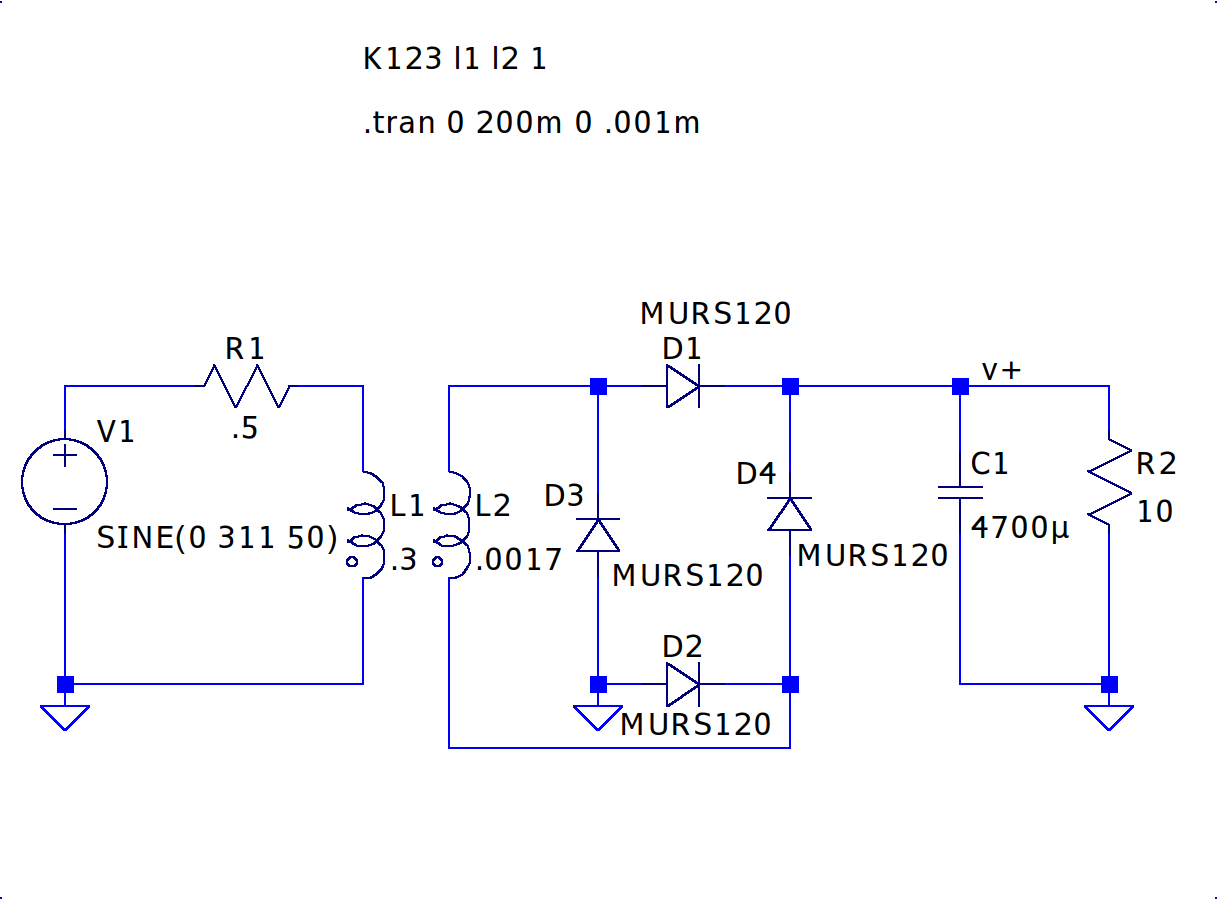
\includegraphics[width=0.8\linewidth]{figuras/fuentes1_circuito.png}
	\caption{Fuente no regulada.}
	\label{fuente1}
\end{figure}


\begin{figure}
	\centering
	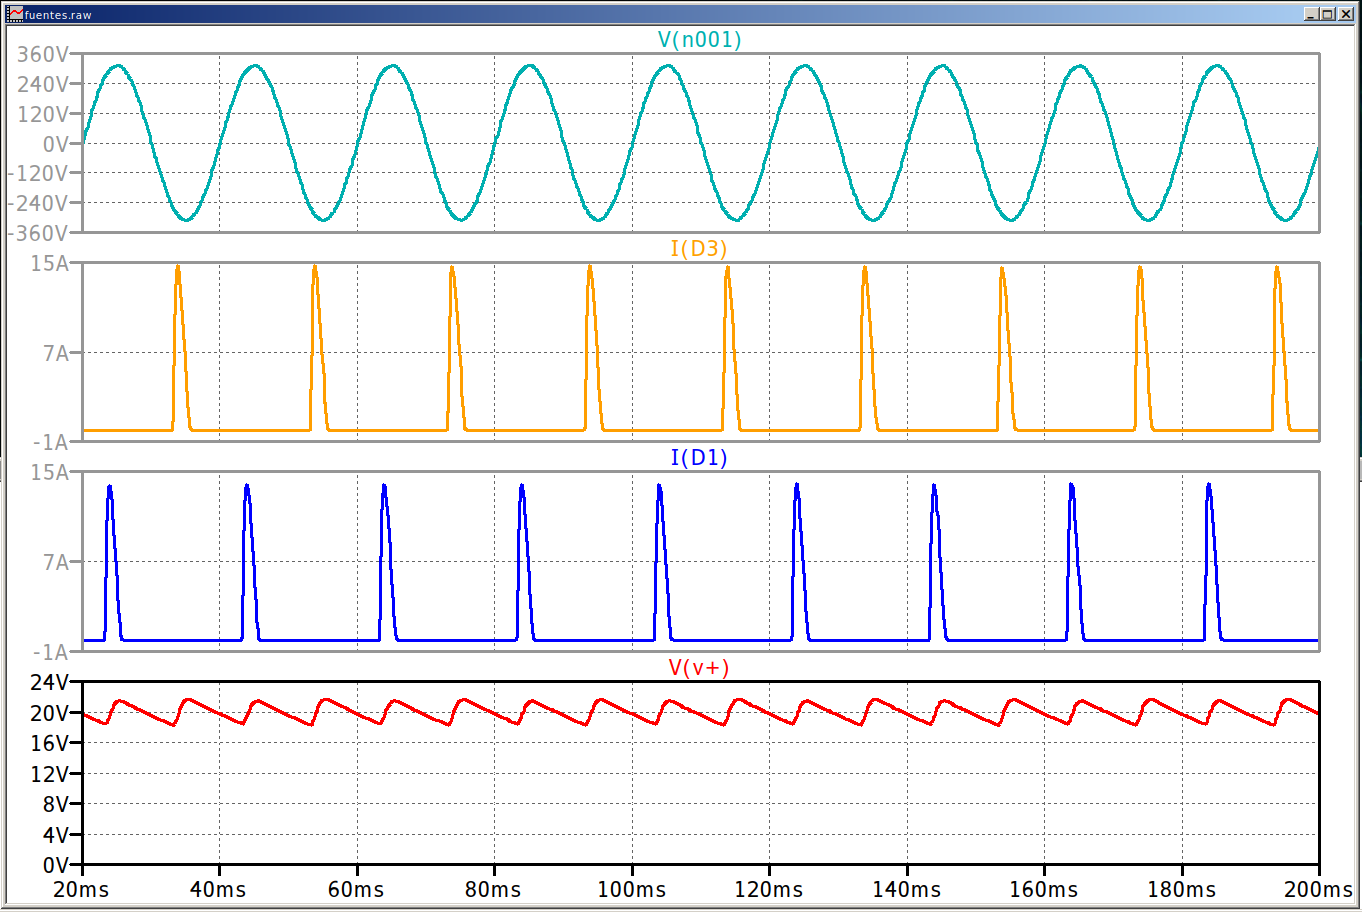
\includegraphics[width=0.8\linewidth]{figuras/fuentes1_curva.png}
	\caption{Simulación de la fuente de la figura \ref{fuente1}.}
	\label{fuente2}
\end{figure}

\subsection{Fuente regulada serie}

{\hspace{10pt}} En la figura \ref{fuente3} se muestra el circuito de una fuente regulada de tensión básica. La fuente no regulada primaria se modeliza con la fuente $V_1$ de $15V$ de valor medio con una señal senoidal superpuesta de $1\hat{V}$ y $100Hz$, simulando el ripple, y una resistencia en serie de $1.2\Omega$. El sensado de la salida se realiza a través de las resistencias $R_1$ y $R_2$ y la referencia de tensión la da el diodo zener con las resistencias $R_4$ y $R_3$, siendo esta última variable para realizar el ajuste buscado ($V_o=9V$ en este caso). El operacional es el encargado de realizar la comparación entre la nuestra de las salida y la referencia y del manejo de la base del transistor tipo Darlingnton $TIP120$, que es el dispositivo que controla la corriente de salida.

 El transistor Darlingnton se implementa como un subcircuito referido a una biblioteca específica agregada (en este caso se utiliza la directiva Spice \emph{.lib 1propia.lib}). El elemento circuital Darlington no está incluido en la biblioteca gráfica disponible, por lo que hay que generarlo a través de la herramienta New Symbol presente en la pestaña File del software LTSpice y luego vincularlo al subcircuito de biblioteca correspondiente.  
 
 \begin{figure}
 	\centering
 	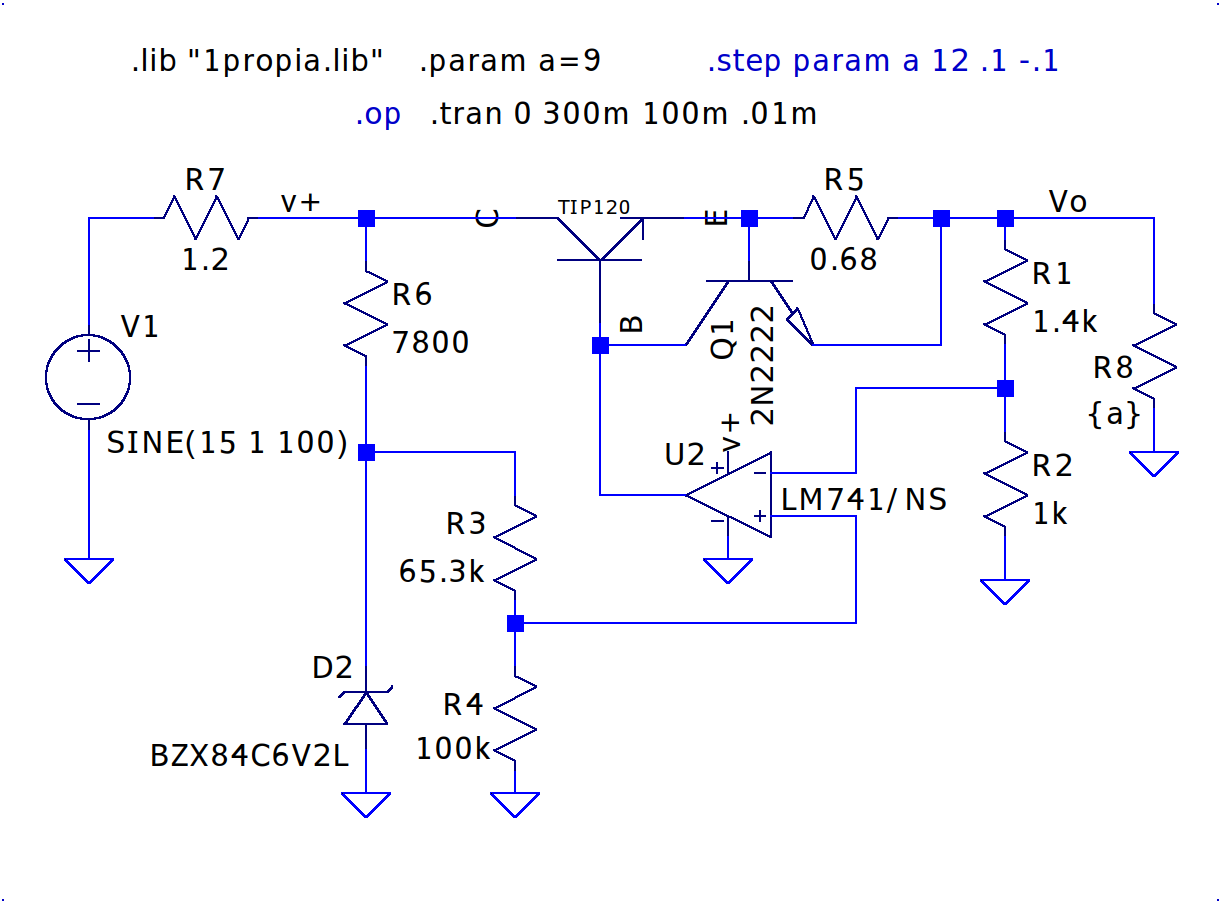
\includegraphics[width=0.8\linewidth]{figuras/fuentes2_circuito.png}
 	\caption{Fuente regulada serie.}
 	\label{fuente3}
 \end{figure}
 
 
 El Transistor $Q_1$ junto con la resistencia $R_5$ son los encargados de dar la protección contra cortocircuitos limitando la máxima corriente posible de salida.
 
 Los resultados obtenidos con la directiva punto de operación en continua \emph{.op}, utilizando $R_8$ igual a $1K\Omega$, a $100\Omega$ y a $10\Omega$, dio como resultado $V_o$ igual a $9.005V$, a $9.004V$ y a $8.9876$ respectivamente. Estos resultados demuestran una buena regulación de  tensión en un rango de corrientes de salida que van de valores muy bajos $\approx 9mA$ hasta $\approx 0.9A$. 
 
 Para realizar un gráfico detallado de la curva de regulación de salida se utiliza una variación de la resistencia de carga $R_8$ entre $12\Omega$ y $0.1\Omega$ en pasos de $0.1\Omega$, a través de la directiva \emph{.step param a 12 .1 .1}  en conjunción con la directiva \emph{.op}. En la figura \ref{fuente4} se muestra el gráfico de $V_o$ en función de la corriente de carga $I(R_8)$, en ella se ve que para corrientes menores a $1.154A$ la tensión de salida se mantiene regulada en $\approx 9V$ y que a partir de esa corriente comienza a actuar el circuito de protección contra cortocircuitos , limitando la corriente a $1.165A$. 
 
Para cuantificar la incidencia del ripple de la entrada en la salida se realiza la simulación temporal \emph{.tran} a máxima carga $\approx 1A$ ($R_8=9\Omega$). En la figura \ref{fuente5} se muestran la entrada $V(v+)$ y la salida $V(Vo)$, se puede observa en ella que $V(v+)$ tiene un valor medio de $13.8V$ y una variación pico a pico de $1.97V$ y que en la salida esa variación de ve atenuada a un valor pico a pico de $30.5mV$, regulando su valor medio en $9V$.

\begin{figure}
	\centering
	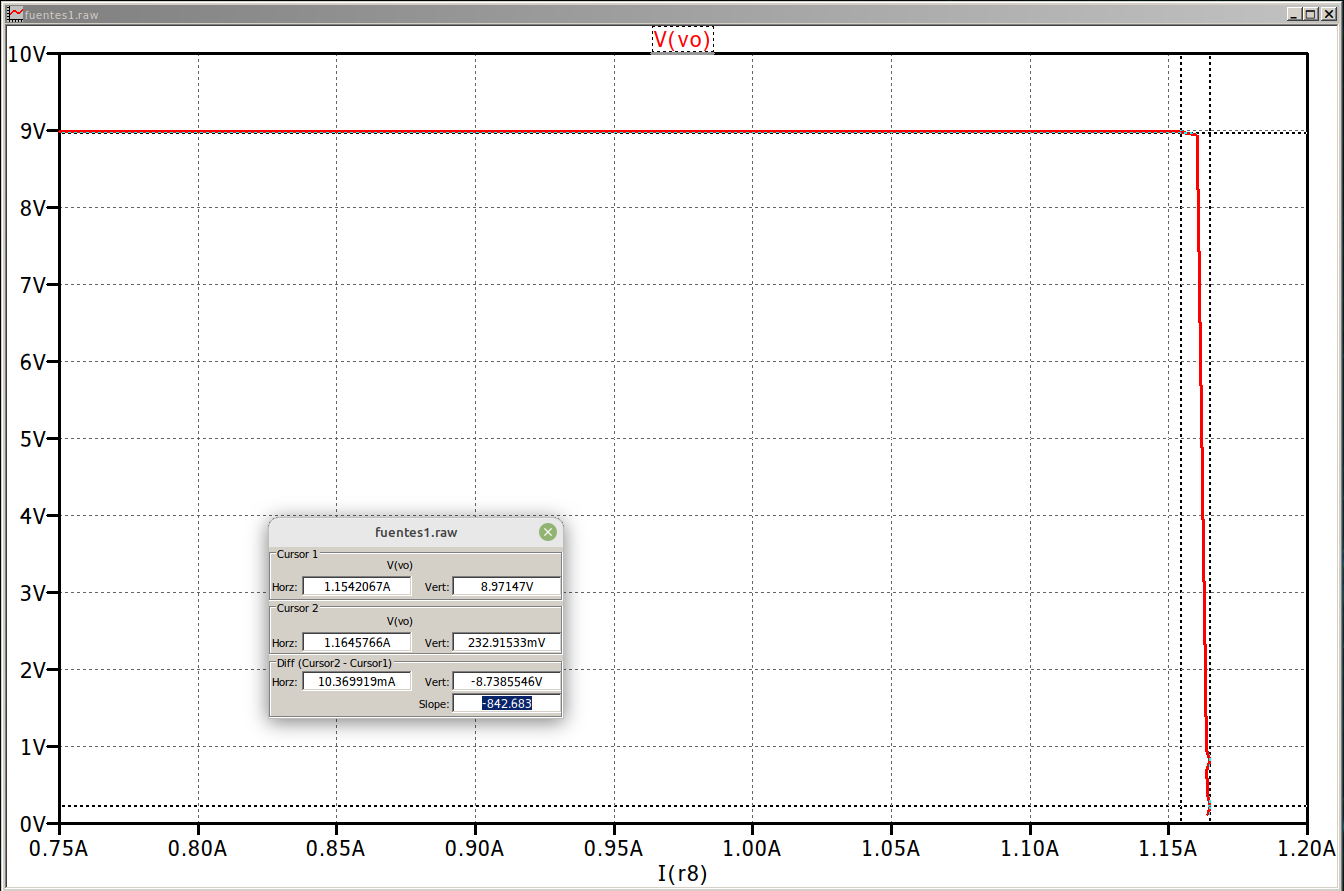
\includegraphics[width=0.8\linewidth]{figuras/fuentes2_curva2.png}
	\caption{Curva de regulación de salida del circuito de la figura \ref{fuente3}.}
	\label{fuente4}
\end{figure}

\begin{figure}
	\centering
	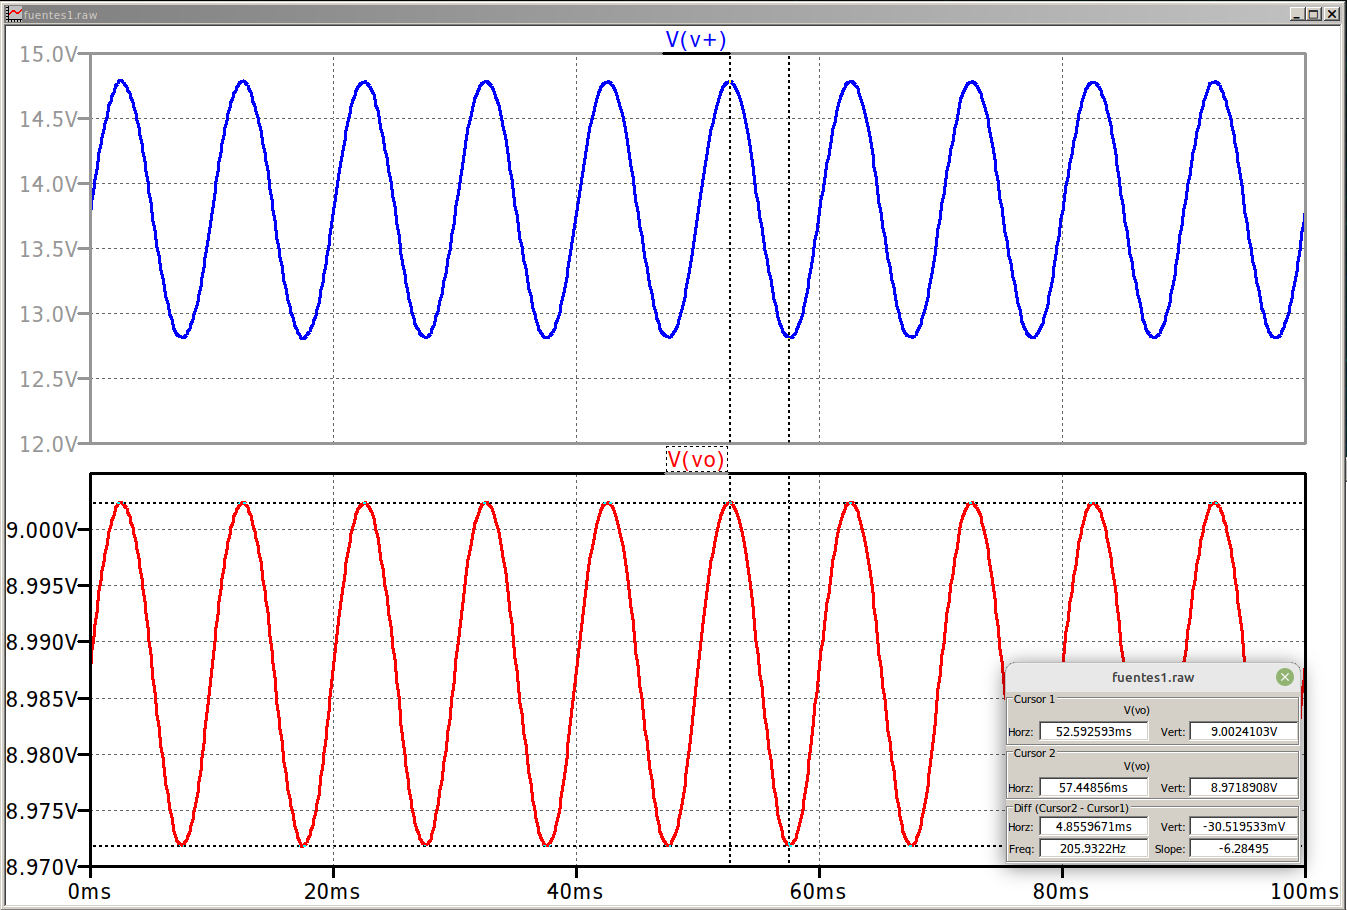
\includegraphics[width=0.8\linewidth]{figuras/fuentes2_curva1.png}
	\caption{Fuente regulada serie. Atenuación del ripple de entrada}
	\label{fuente5}
\end{figure}

\subsection{Fuentes conmutadas}

{\hspace{10pt}} En la figura \ref{fuente6} se muestran  dos configuraciones teóricas de fuentes conmutadas. 

El circuito de la parte superior ilustra el regulador básico denominado \emph{step-down} o \emph{buck}. En este circuito la llave controlada $S_1$ se ubica en serie entre la fuente primaria  de continua $V_{i1}$ y el circuito de salida. La llave se controla por medio de la fuente pulsada $V_p$ conectando y desconectando $V_{i1}$ al ritmo de su frecuencia y de su ciclo de trabajo. Cuando la llave está cerrada la entrada $V_{i1}$ se aplica al circuito de salida permitiendo el flujo de corriente hacia la carga a través del inductor $L_1$, manteniéndose el diodo $D_1$ cortado. Cuando la llave se abre la energía almacenada en el inductor sostiene la corriente a través de la carga, cerrando el circuito por medio de la conducción del diodo $D_1$. El valor de tensión de continua de la salida siempre es menor que el valor de la entrada y depende en forma directa del ciclo de trabajo $c_t$ de la fuente $V_p$, siendo $c_t$ la proporción del período de la fuente $V_p$ en que la llave están conduciendo.

 
 Por otro lado en la parte inferior se muestra el regulador básico denominado \emph{step-up} o \emph{boost}. En este circuito se modifican las posiciones de la llave controlada $S_2$, el diodo $D_2$ y el inductor $L_2$. En este caso cuando la llave $S_2$ está cerrada  el inductor $L_2$ almacena energía a través de la fuente de continua $V_{i2}$, con el diodo $D_2$ cortado. Luego cuando la llave $S_2$ se abre el inductor continúa conduciendo a través del diodo $D_2$ entregando la energía almacenada en el ciclo anterior a la carga. El valor de tensión de continua de la salida siempre es mayor que el valor de la entrada y depende en forma inversa  de $1-c_t$.
 
 En ambos casos, controlando el ciclo de trabajo de la llave por medio de un sistema realimentado que sense la salida se puede implementar un regulador de tensión conmutado. Las llaves  controladas se pueden implementar con Transistores Bipolares o MOSFETs.
 
  \begin{figure}
  	\centering
  	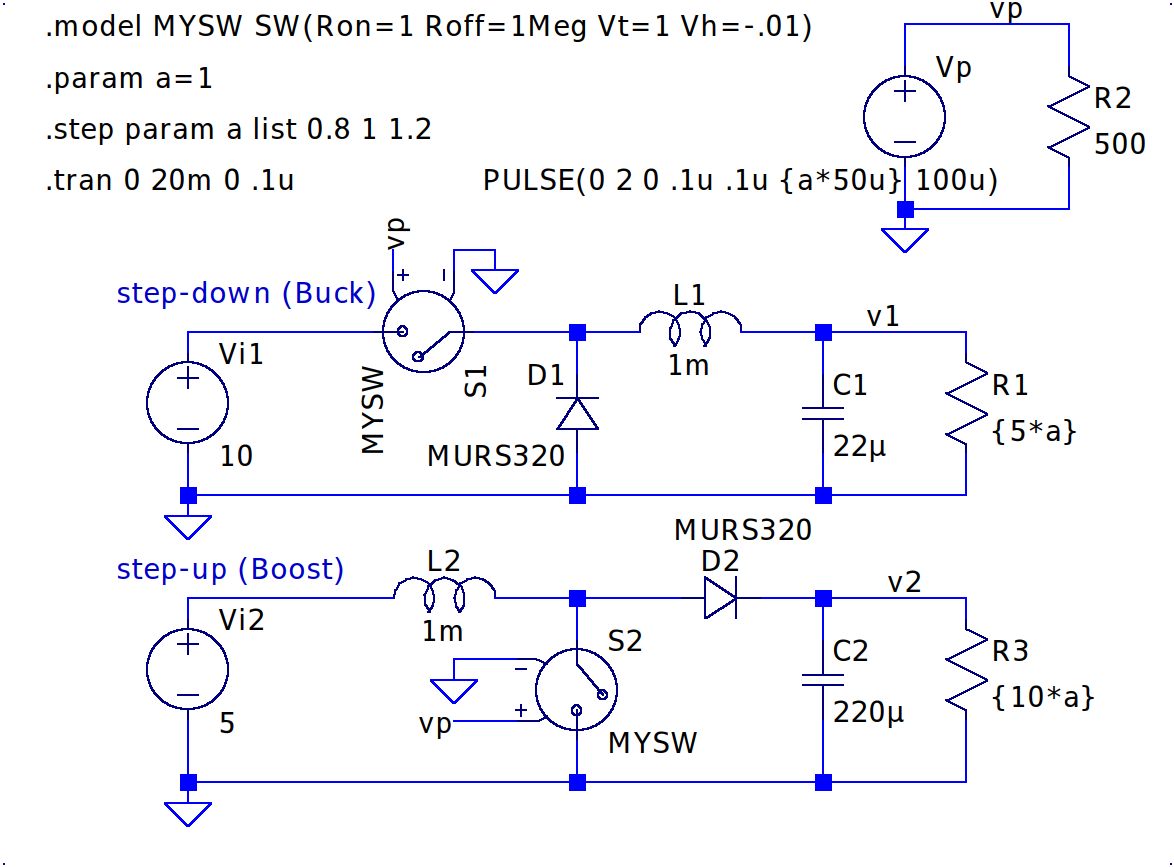
\includegraphics[width=0.8\linewidth]{figuras/fuentes3_circuito.png}
  	\caption{Fuentes conmutadas \emph{step-down} y \emph{step-up}.}
  	\label{fuente6}
  \end{figure}
 
 
 En la figura \ref{fuente7} se muestra la simulación temporal de los circuitos presentados para el caso en que el parámetro $a=1$, es decir que el ciclo de trabajo de la fuente $V_p$ es del 50\% y las cargas son $R_1=5\Omega$ y $R_3=10\Omega$. En ella se ve en la parte inferior las salidas $V(v_1)$ y $V(v_2)$ y en la superior las corrientes de los inductores $L_1$ y $L_2$. Se ve que las tensiones promedio a la salida coinciden con lo esperado, menor que la fuente de entrada en $V(v_1)$ y mayor que la entrada en $V(v_2)$ y que las corrientes en los inductores no se cortan dentro del ciclo de trabajo.
 
 En la figura \ref{fuente8} se muestran las tensiones de salida de ambos circuitos variando el ciclo de trabajo, mediante la directiva \emph{.step param a list 0.8 1 1.2}, que realiza la simulación para los casos de ciclo de trabajo del 40\%, del 50\% y del 60\% respectivamente. Es de notar que se varió también las resistencias de carga de los circuitos en función de $a$ para que las corrientes promedio de carga se mantengan aproximadamente constantes para cada valor de $a$. Se ve en ambos casos el aumento del valor promedio de la salida en función del aumento del ciclo de trabajo.
 
 \begin{figure}
 	\centering
 	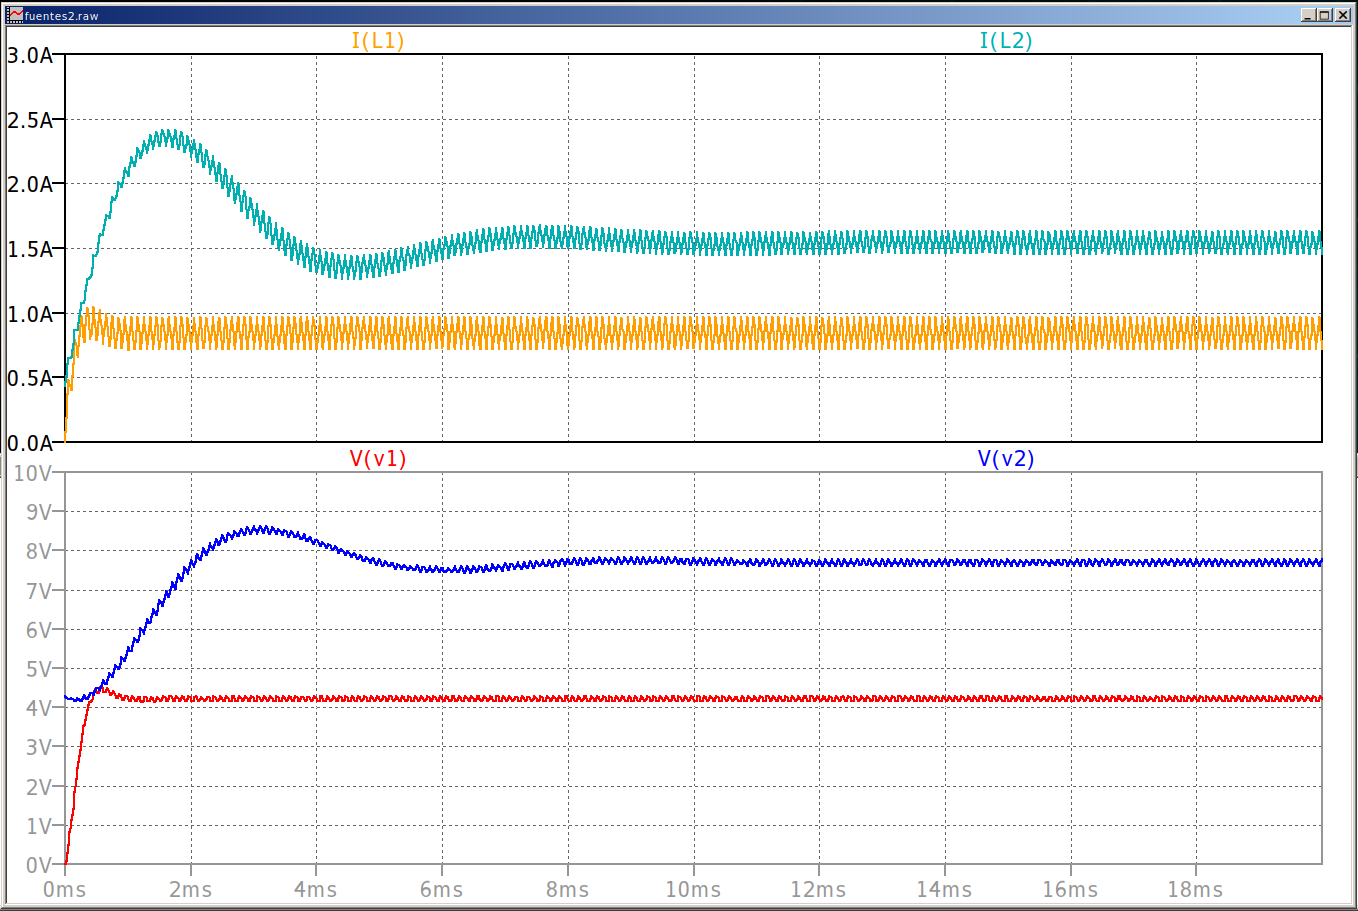
\includegraphics[width=0.8\linewidth]{figuras/fuentes3_curva1.png}
 	\caption{Tensiones de salida y corrientes de los inductores para ciclo de trabajo del 50\% en los circuitos de la figura \ref{fuente6}.}
 	\label{fuente7}
 \end{figure}
 
 \begin{figure}
 	\centering
 	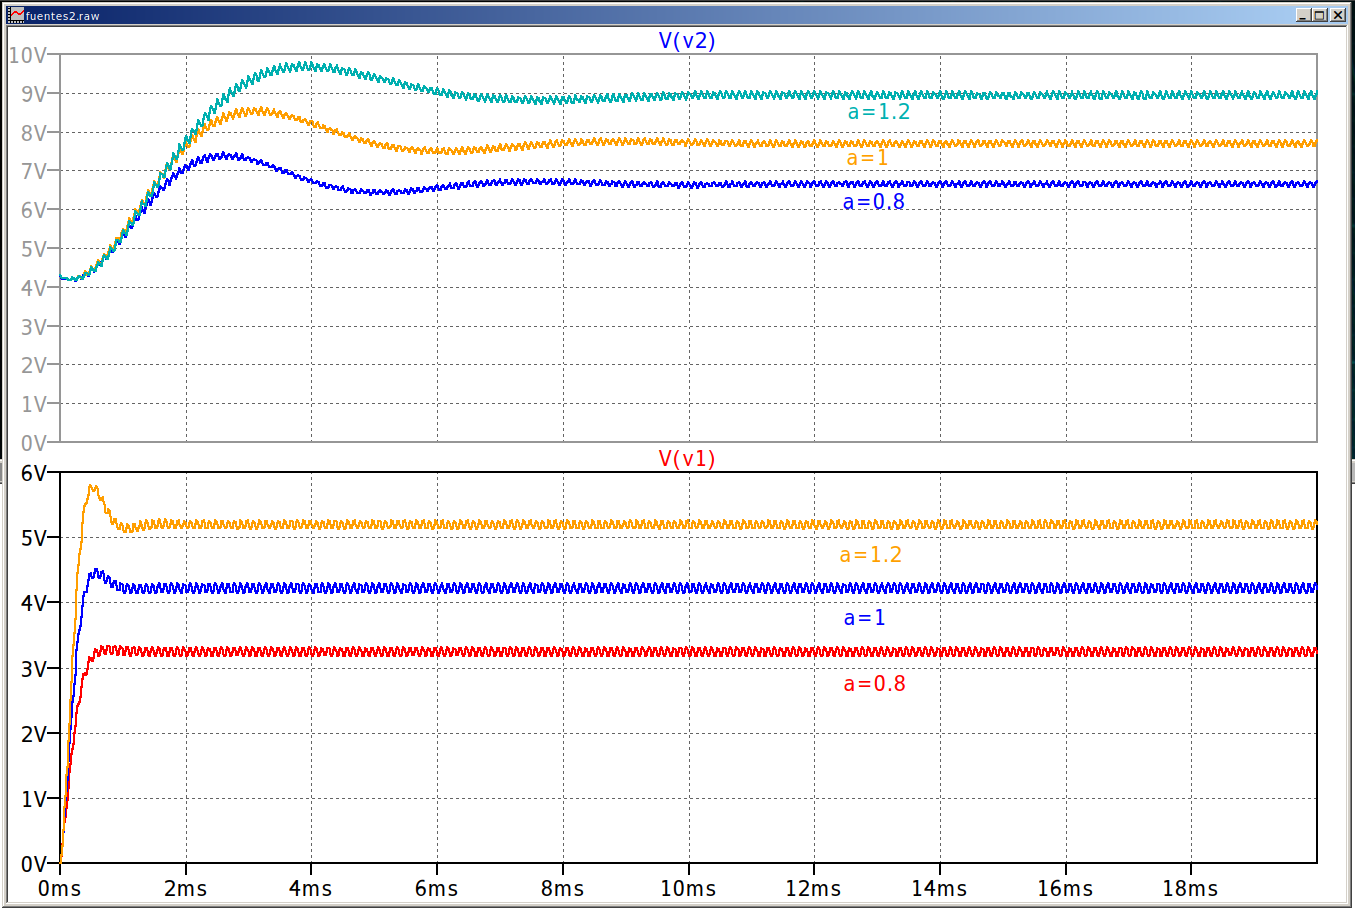
\includegraphics[width=0.8\linewidth]{figuras/fuentes3_curva3.png}
 	\caption{Tensiones de salida para ciclos de trabajo del 40\%, 50\% y 60\% ($a=0.8$, $a= 1$ y $a=1.2$ respectivamente), en los circuitos de la figura \ref{fuente6}.}
 	\label{fuente8}
 \end{figure}
 
 \section{Amplificadores Sintonizados}
 
 {\hspace{10pt}} Los amplificadores sintonizados pueden definirse como una red selectiva en frecuencia que además amplifica a las señales que sintoniza. Los circuitos más sencillos utilizados son los denominados: "Sintonía Simple" y "Sintonía Escalonada".
 
 \subsection{Sintonía Simple}
 
 {\hspace{10pt}}  El concepto general de amplificador de sintonía simple puede asimilarse a un amplificador que alimenta a una carga $RLC$ paralelo. La resonancia de la red $LC$ determina la frecuencia central de la banda de paso $f_o= \displaystyle \frac{1}{2 \pi \sqrt{LC}}$ y el factor de calidad $Q=\displaystyle \frac{R}{2 \pi f_o L}=2 \pi f_o C R$ determina el ancho de banda $B=\displaystyle \frac{f_o}{Q}$. La ganancia del amplificador a la frecuencia central de resonancia depende directamente de $R$. 
 
 En algunos casos esta solución no es satisfactoria para los requerimientos de ancho de banda y selectividad buscados. Para mejorar estas características se utiliza el concepto de sintonía sincronizada, que son etapas individuales idénticas en $f_o$ y $Q$ de sintonía simple dispuestas en cascada. Dando como resultado, la misma frecuencia central $f_o$ y un ancho de banda total de $B_t=B\sqrt{2^{\frac{1}{n}}-1}$, siendo $n$ el número de etapas y $B$ el ancho de banda de cada etapa individual.
 
 El circuito de la figura \ref{sintonia1} muestra un circuito de sintonía sincronizada de dos etapas. La etapa sintonizada de entrada está compuesta por $L1$, $C_1$ y por la resistencia total equivalente en paralelo con la red $L_1C_1$. 
 
 La entrada de señal $V_3$ está acoplada a la entrada del amplificador diferencial a través del transformador reductor $L_1-L_2$, implementado con la directiva \emph{.K12 L1 L2 1} que simula el acoplamiento inductivo entre dos inductores con un $K=1$ ideal. Este transformador se suele colocar para atenuar los efectos en el resonador paralelo de las capacidades y resistencias que presenta el transistor $Q_1$.
 
 En el colector del transistor $Q_2$ se ubica la segunda etapa sintonizada acoplada por el transformador elevador $L_3-L_4$ y dada por el paralelo de $L_4$, $C_4$ y por la resistencia total equivalente en paralelo con la red $L_4C_4$. 
 
 Para lograr la sintonía exacta se utilizaron capacitores variables
de ajuste en $C_1$ y $C_4$.
 
 En la figura \ref{sintonia2} se muestra la simulación de la respuesta en frecuencia del circuito de la figura \ref{sintonia1}. 
 
 En la parte inferior se grafica: $V(b)=\displaystyle \frac{V(b)}{V_3}=\displaystyle \frac{V(b)}{1V}$ que representa la respuesta en frecuencia de la primera etapa referida al secundario del transformador $L_1-L_2$; $\displaystyle \frac{V(vo)}{V(b)}$ que representa la respuesta de la segunda etapa y $V(vo)$ que representa la trasferencia total del amplificador con $V_3=1V$. Del gráfico y utilizando los cursores se obtuvo que: la primera etapa presenta una frecuencia central $f_{o1}=454.99KHz$, un ancho de banda $B_1=16.28KHz$ y un $Q_1=27.95$ y que la segunda etapa tiene una frecuencia central $f_{o2}=454.87KHz$, un ancho de banda $B_2=15.76KHz$ y un $Q_2=28.86$. Con respecto a la transferencia total la frecuencia central es $f_{o}=454.92KHz$ y su ancho de banda $B_t=10.3KHz$, siendo su ganancia a frecuencia central de $28.27dB$. Estos resultados coinciden muy aproximadamente con los predichos teóricamente.
 
 En la parte superior se grafican las mismas curvas normalizadas a $0dB$, en ella se ve que ambas etapas individuales tienen transferencias prácticamente iguales y ambas en cascada redundan en una transferencia total más selectiva y con menor ancho de banda.  
 
 \begin{figure}
 	\centering
 	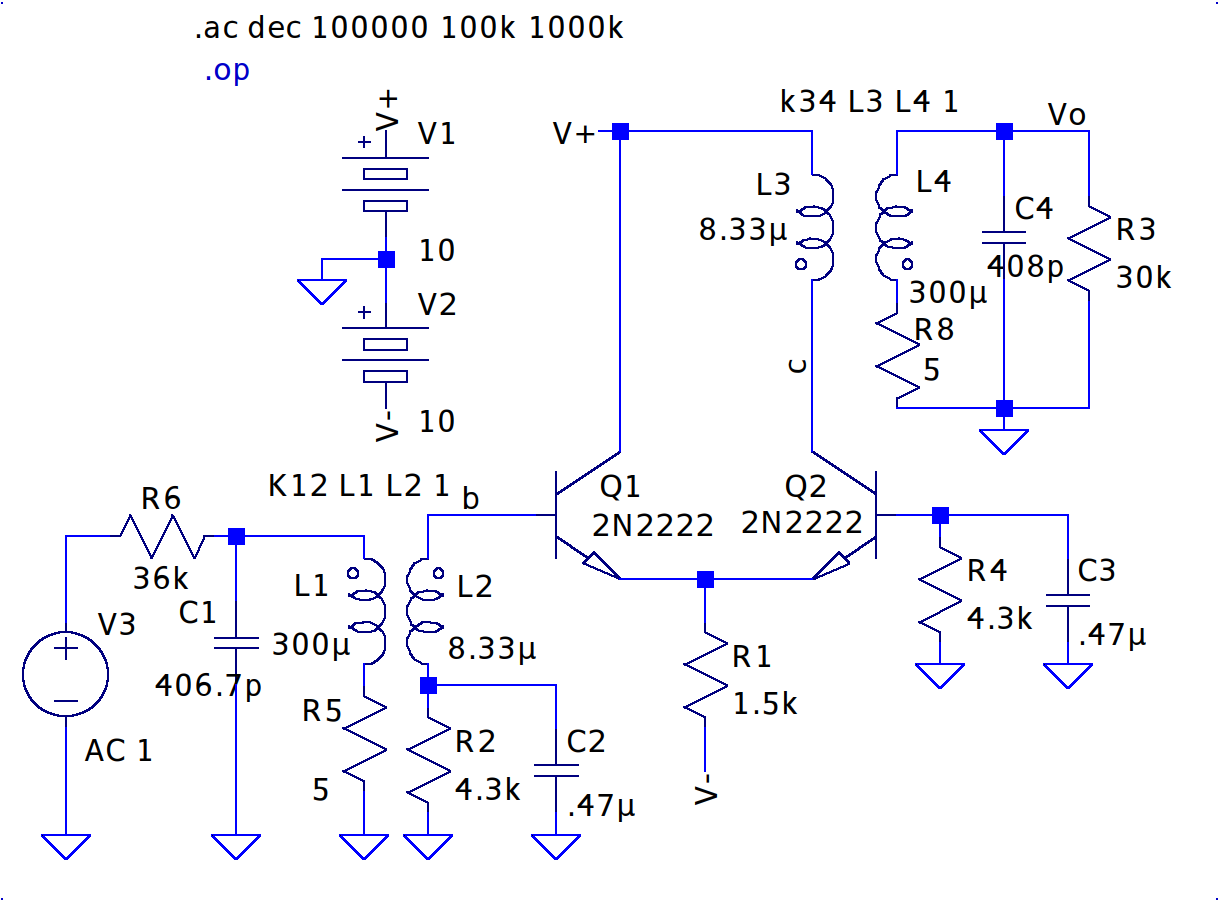
\includegraphics[width=0.8\linewidth]{figuras/sintonia_circuito.png}
 	\caption{Amplificador sintonizado con dos etapas de sintonía simple.}
 	\label{sintonia1}
 \end{figure}
 
 \begin{figure}
 	\centering
 	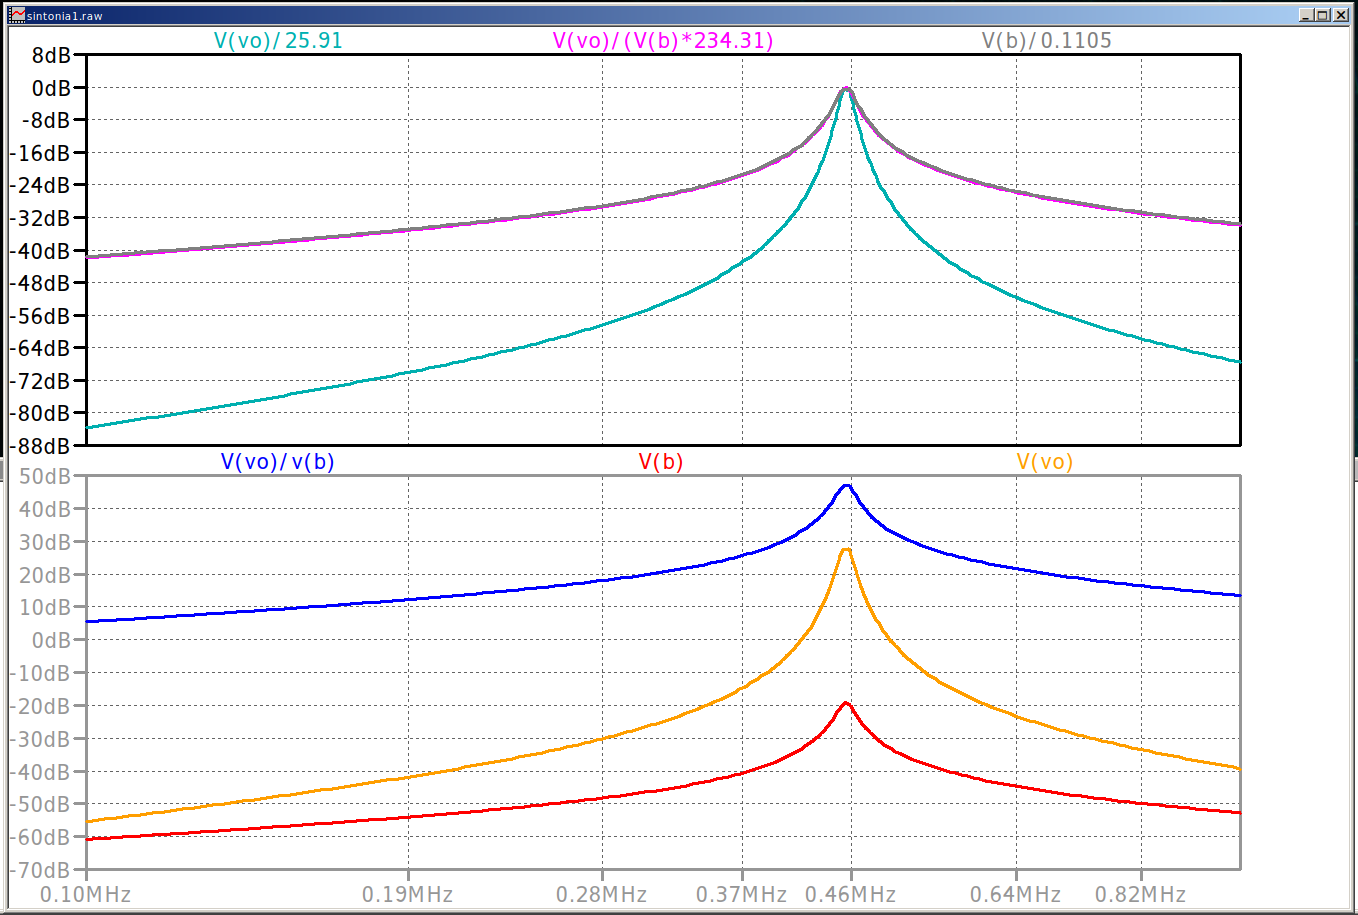
\includegraphics[width=0.8\linewidth]{figuras/sintonia_curva1.png}
 	\caption{Respuesta en frecuencia del circuito de la figura \ref{sintonia1}.}
 	\label{sintonia2}
 \end{figure}
 
 \subsection{Sintonía Escalonada}
 
 {\hspace{10pt}} Si se desea una banda de paso más plana y mejoras adicionales en la selectividad se puede utilizar el concepto de sintonía escalonada. Para dos etapas se diseña para que las frecuencias centrales ya no sean iguales sino desplazadas levemente una hacia las frecuencias más bajas y la otra en el sentido contrario. Utilizando el mismo circuito de la figura \ref{sintonia1}, pero modificando $C_1=401.6pF$ y $C_2=414.3pF$ para el desplazamiento de las frecuencias y modificando las resistencias $R_6=220k$ y $R_3=82K$ para adaptar el ancho de banda de cada etapa se obtienen los resultados de simulación mostrados en la figura \ref{sintonia3}.
 
Al igual que en caso anterior, en la parte inferior se grafica: $V(b)$ que representa la respuesta en frecuencia de la primera etapa; $\displaystyle \frac{V(vo)}{V(b)}$ que representa la respuesta de la segunda etapa y $V(vo)$ que representa la trasferencia total del amplificador. Del gráfico y utilizando los cursores se obtuvo que: la primera etapa presenta una frecuencia central $f_{o1}=457.79KHz$ y un ancho de banda $B_1=7.05KHz$ y que la segunda etapa tiene una frecuencia central $f_{o2}=451.38KHz$ y un ancho de banda $B_2=7.46KHz$. Con respecto a la transferencia total la frecuencia central es $f_{o}=455.05KHz$ y su ancho de banda $B_t=9.0KHz$, siendo su ganancia a frecuencia central de $21.13dB$.

En la parte superior se grafican las mismas curvas normalizadas a $0dB$, en ella se ve que ambas etapas individuales tienen transferencias parecidas pero desplazadas en frecuencia y ambas en cascada contribuyen en una transferencia total más plana en su banda de paso y selectiva en sus flancos y con menor ancho de banda.  

 \begin{figure}
 	\centering
 	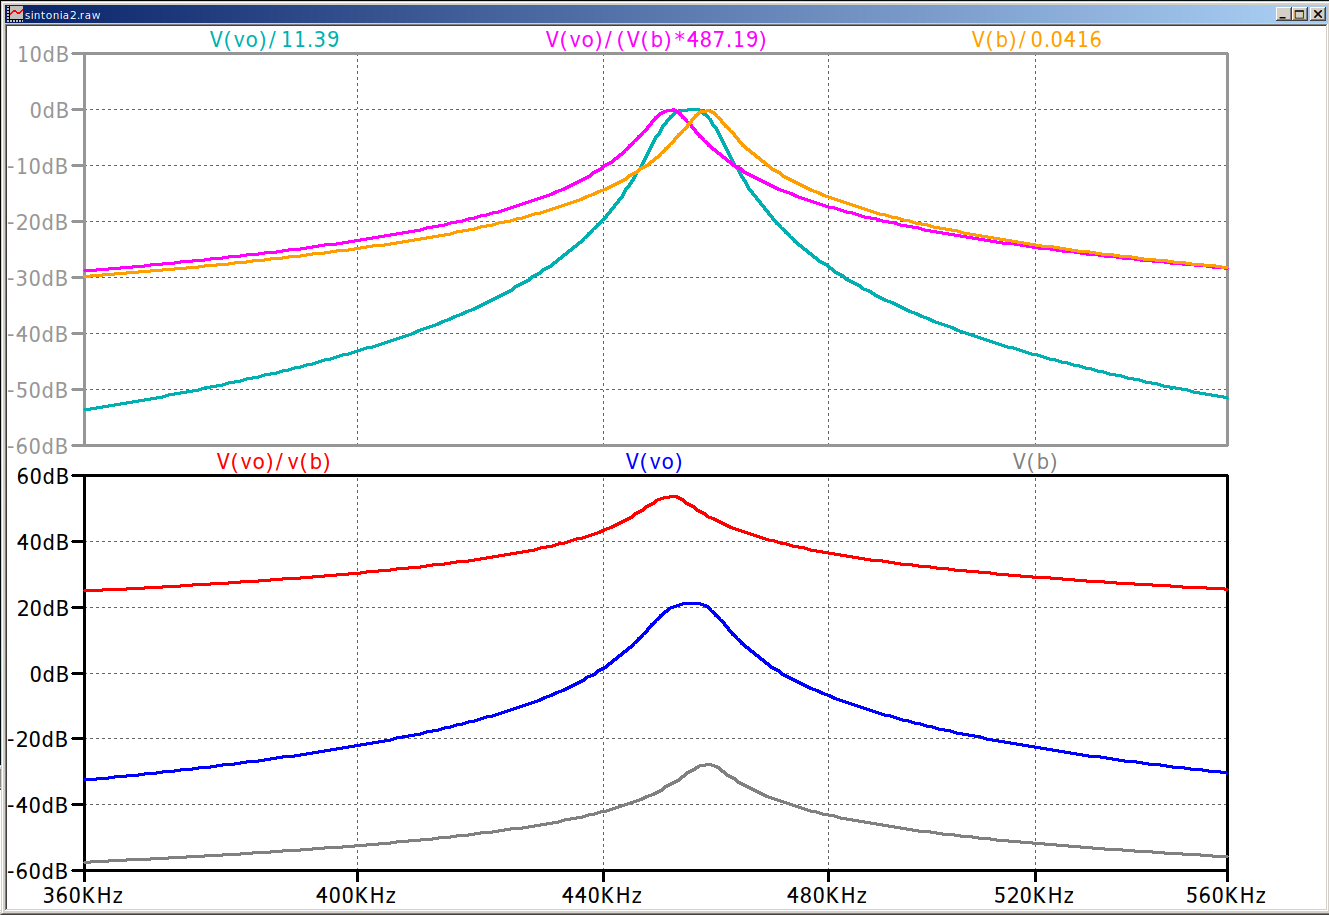
\includegraphics[width=0.8\linewidth]{figuras/sintonia_curva2.png}
 	\caption{Respuesta en frecuencia del circuito de la figura \ref{sintonia1} modificado para sintonía escalonada.}
 	\label{sintonia3}
 \end{figure}
 
 \section{Dispositivos de disparo}
 
 {\hspace{10pt}} Los dispositivos de disparo no tienen un modelo específico SPICE, para utilizarlos como parte de un circuito deben ser definidos como subcircuitos mediante un modelo apropiado. Los fabricantes suelen proveer libremente las bibliotecas de los subcircuitos que modelizan sus dispositivos. LTSpice provee los símbolos circuitales de SCRs, TRIACs e IGBTs, para poder ser usados en sus circuitos se debe referenciar cada símbolo a un subcircuito perteneciente a una biblioteca disponible. En caso de símbolos de dispositivos no disponibles en LTSpice, tal como los UJTs u otros, se deben crear los símbolos mediante el editor gráfico disponible y luego referenciarlos a la biblioteca específica.
 
  
  \subsection{Tiristores y TRIACs}
  
   {\hspace{10pt}} Los circuitos mostrados en la figura \ref{disparo1} representan el método básico de control de potencia de AC a una carga por medio de un Tiristor (SCR), en el circuito de la izquierda, y a través de un TRIAC, en el de la derecha.
   
   El disparo de los dispositivos se logra por medio de las fuentes pulsadas $V_2$ y $V_3$ sincronizadas con la red de corriente alterna $V_1$ y conectadas a las compuertas de los dispositivos correspondientes a través de las resistencias $R_2$ y $R_4$. Cuando los dispositivos se disparan, en el semiciclo positivo de la fuente de AC el SCR y en ambos semiciclos el TRIAC, las cargas $R_1$ y $R_3$ conducen la corriente entregada por la fuente de AC hasta que esta se extingan al final del semiciclo produciéndose el corte del dispositivo. 
   
   En la figura \ref{disparo2} se muestra la respuesta temporal de ambos circuitos. La curva inferior representa la red de AC, las tres siguientes corresponden al circuito controlado por el SCR y las tres superiores al controlado por el TRIAC. Con respecto al circuito del SCR, se ve que la fuente $V_2$ produce el pulso de disparo en un tiempo de $2.5ms$ posterior al inicio del semiciclo positivo de la fuente de AC, es decir el ángulo de disparo es de $\theta_d=45^{\circ}$ y por lo tanto el de conducción es de $\theta_c=135^{\circ}$; esto se ve reflejado en las curvas de corriente en la carga $I(R_1)$ y tensión sobre el SCR $V(va)$. En forma similar las tres curvas superiores reflejan el funcionamiento del circuito controlado por el TRIAC, $V_3$ es la fuente de disparo, $I(R_3)$ la corriente en la carga y $V(vb)$ la tensión sobre el TRIAC, en este caso hay conducción en ambos semiciclos de la señal de AC.
   
   En las curvas de la figura \ref{disparo3} se muestran las simulaciones de las corrientes en la carga en ambos casos para tres valores del parámetro $a$, que controla el tiempo de disparo y por lo tanto el ángulo de disparo. Se muestran tres casos particulares: $a=1ms$ que refleja una conducción casi completa dentro del  semiciclo, $a=5ms$ que significa una conducción de la mitad del tiempo y $a=9ms$ una conducción de una muy pequeña fracción dentro del semiperíodo.
   
   \begin{figure}
   	\centering
   	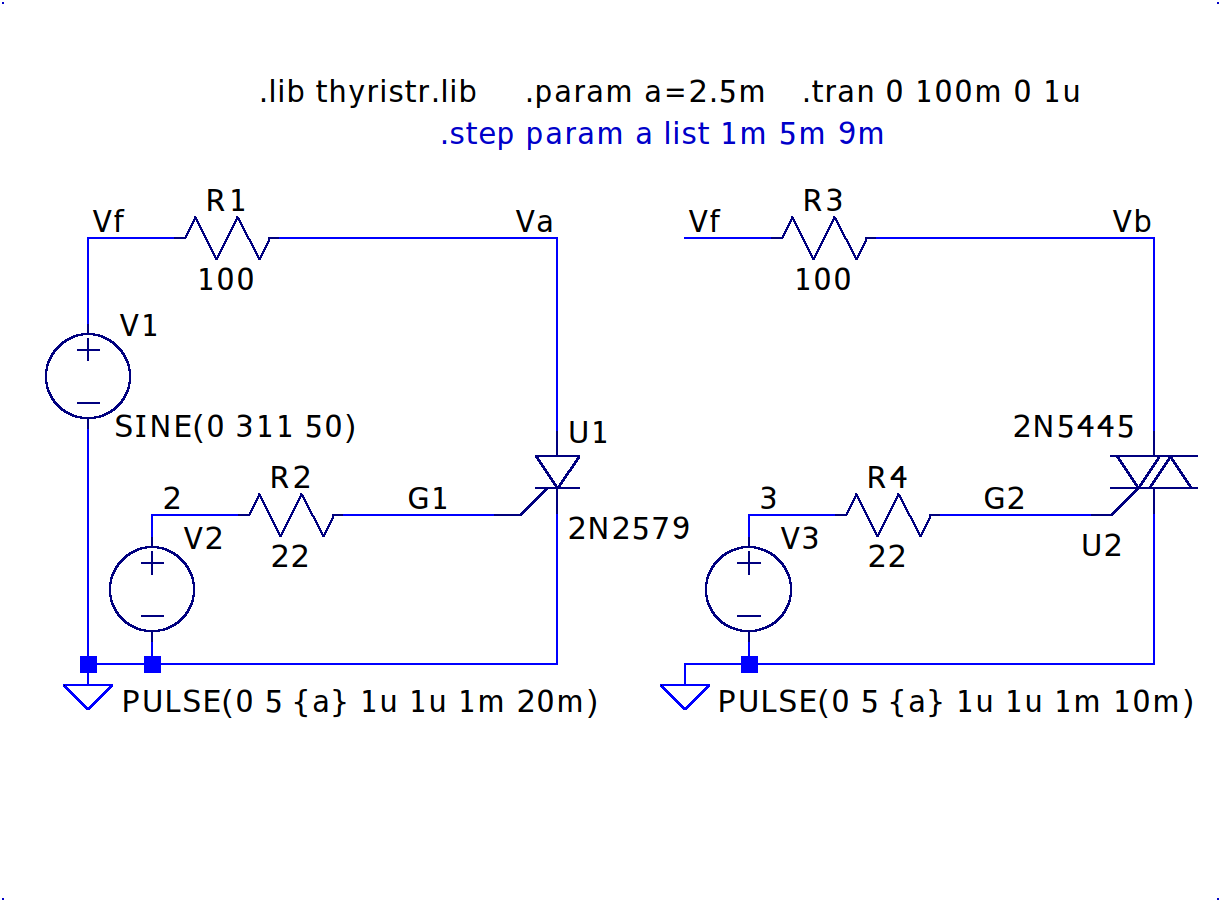
\includegraphics[width=0.8\linewidth]{figuras/tiristor_circuito.png}
   	\caption{Control de potencia de AC en una carga mediante SCR y TRIAC.}
   	\label{disparo1}
   \end{figure}
   
   \begin{figure}
   	\centering
   	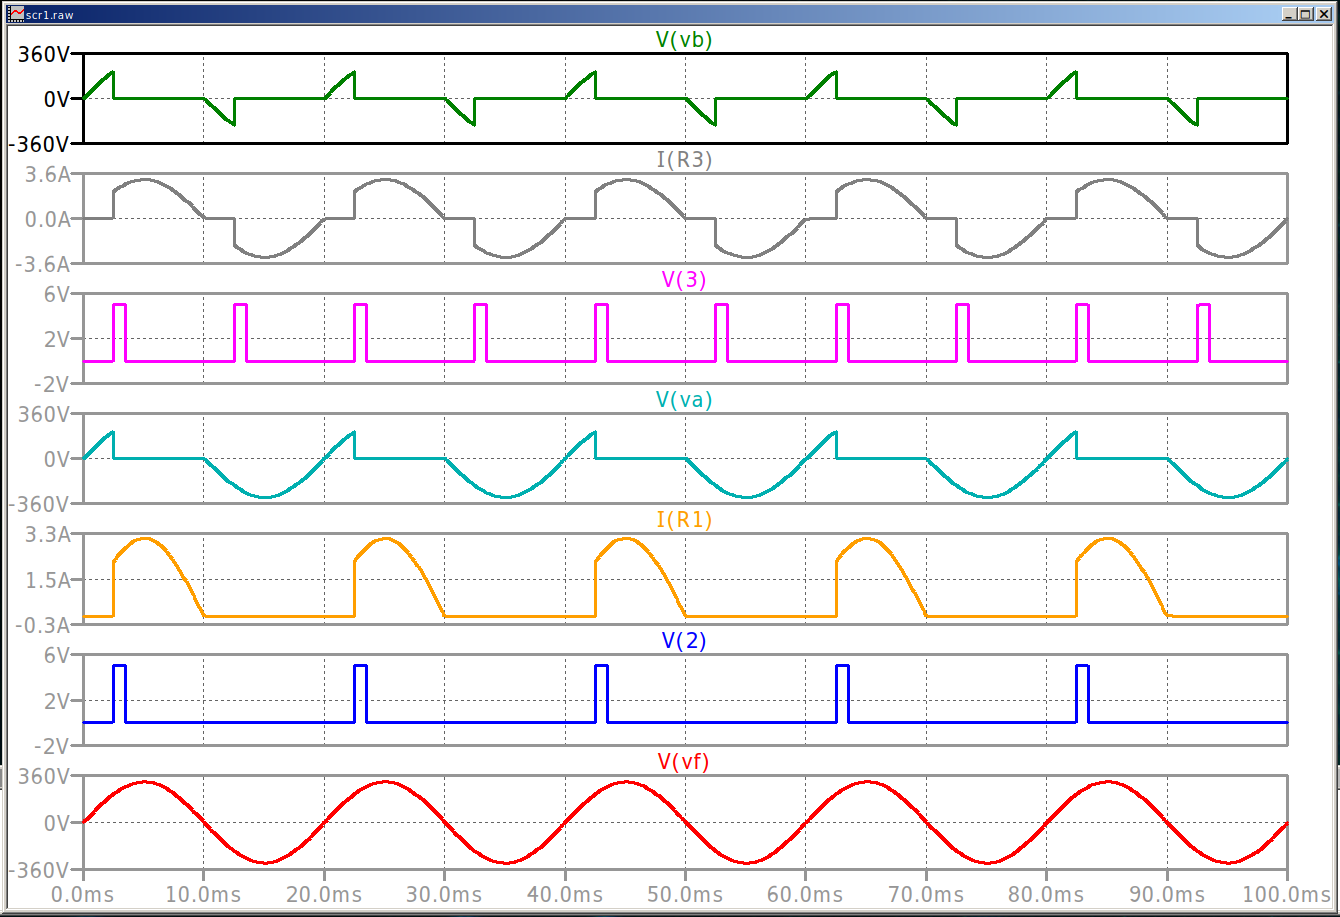
\includegraphics[width=0.8\linewidth]{figuras/tiristor_curva1.png}
   	\caption{Simulación temporal de los circuitos de la figura \ref{disparo1}.}
   	\label{disparo2}
   \end{figure}
   
   \begin{figure}
   	\centering
   	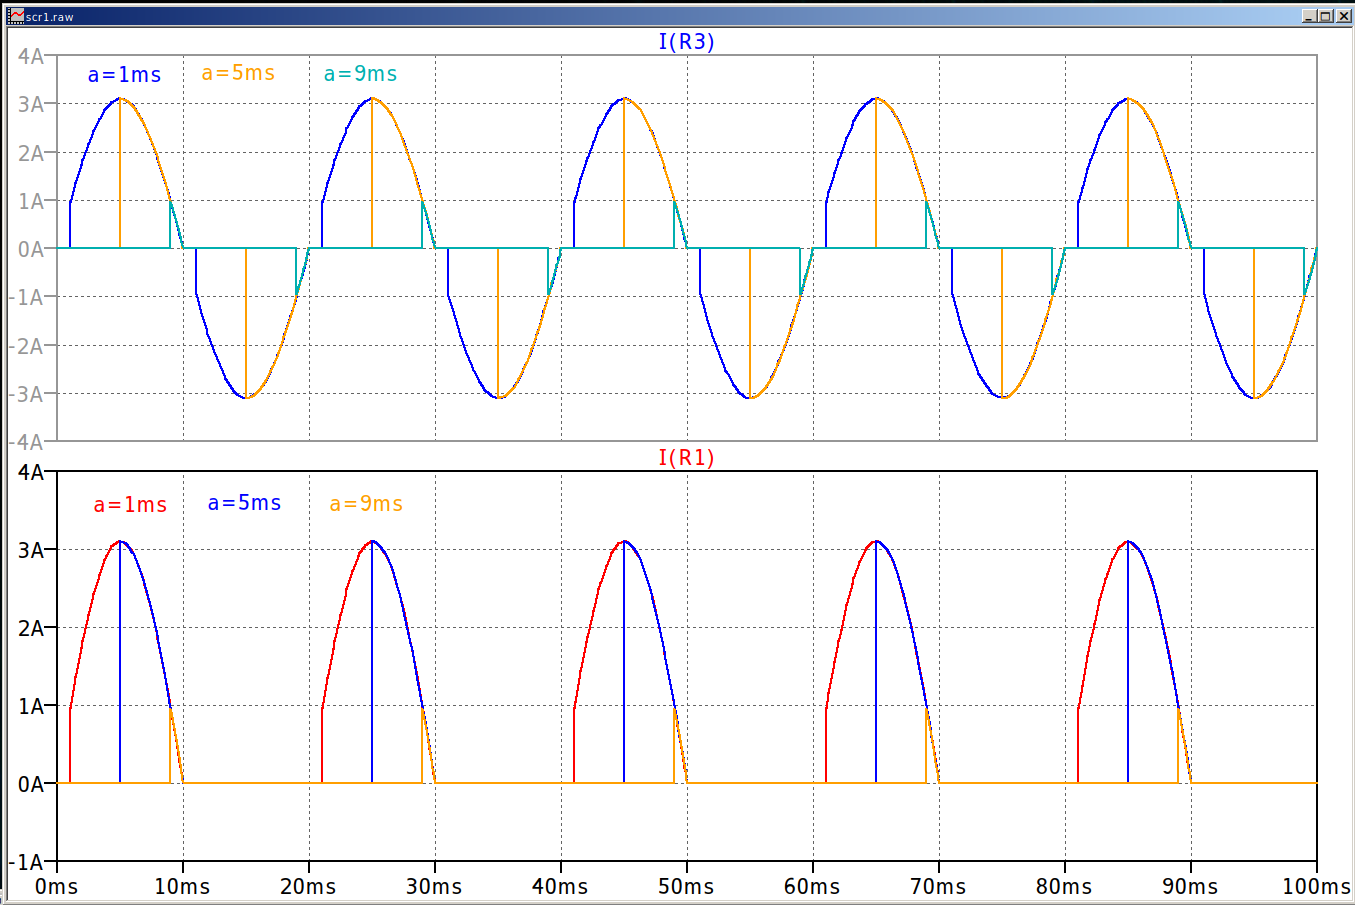
\includegraphics[width=0.8\linewidth]{figuras/tiristor_curva2.png}
   	\caption{Variación del tiempo de conducción en los circuitos de la figura \ref{disparo1}.}
   	\label{disparo3}
   \end{figure}
   
    \subsection{Oscilador de relajación con UJTs}
    
    {\hspace{10pt}} El transistor Unijuntura UJT es un dispositivo que presenta en su curva tensión emisor-base1 en función de la corriente de emisor una zona de resistencia diferencial negativa, que lo hace útil para la implementación de osciladores de relajación. Un ejemplo de este tipo de osciladores es el mostrado en la figura \ref{ujt1}, si la recta de carga  de emisor dada por $V_1=I_eR_1+V_e$ se sitúa en la zona de resistencia negativa del UJT y se coloca un capacitor en paralelo con el emisor se puede lograr la oscilación buscada. El modelo del UJT se obtiene del subcircuito disponible en la librería correspondiente y el símbolo gráfico debe crearse especialmente para el circuito. 
    
    En la figura \ref{ujt2} se muestra la simulación temporal del oscilador. En la curva inferior se grafica la tensión del emisor que está en paralelo con el capacitor $C_1$, allí se ve que en el ciclo de carga del capacitor su tensión evoluciona al ritmo exponencial de un circuito RC típico, ya que el UJT está cortado. Cuando la tensión del capacitor (y del emisor) llega al valor de disparo el UJT conduce fuertemente descargando rápidamente el capacitor hasta que se llega a la tensión de corte del UJT, comenzando nuevamente el ciclo de carga. En la curva superior se muestra el pico de corriente producido cuando conduce el UJT a través de la caída en la resistencia $R_3$ en la base 1.    
    
      \begin{figure}
    	\centering
    	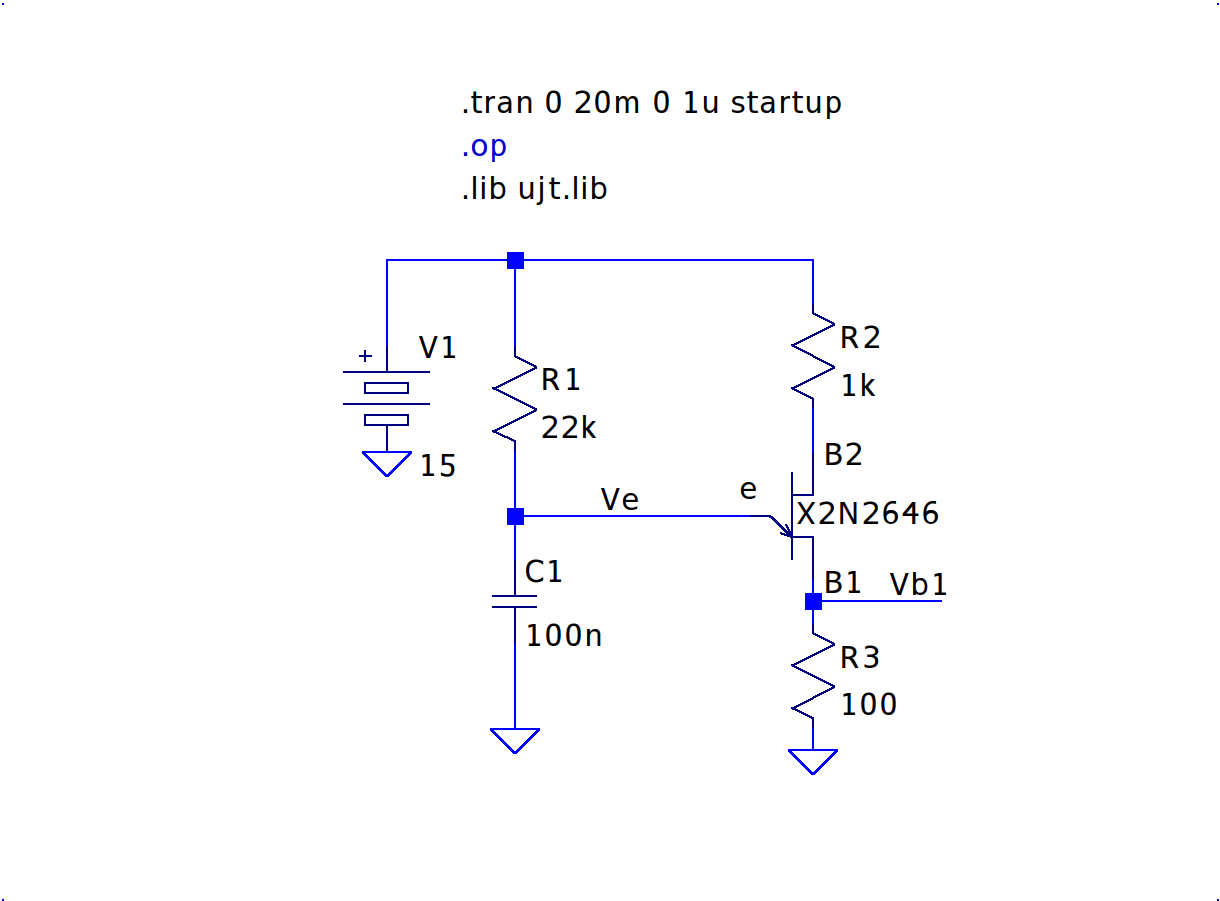
\includegraphics[width=0.8\linewidth]{figuras/oscujt_circuito.png}
    	\caption{Oscilador de relajación con UJT.}
    	\label{ujt1}
    \end{figure}
    
    \begin{figure}
    	\centering
    	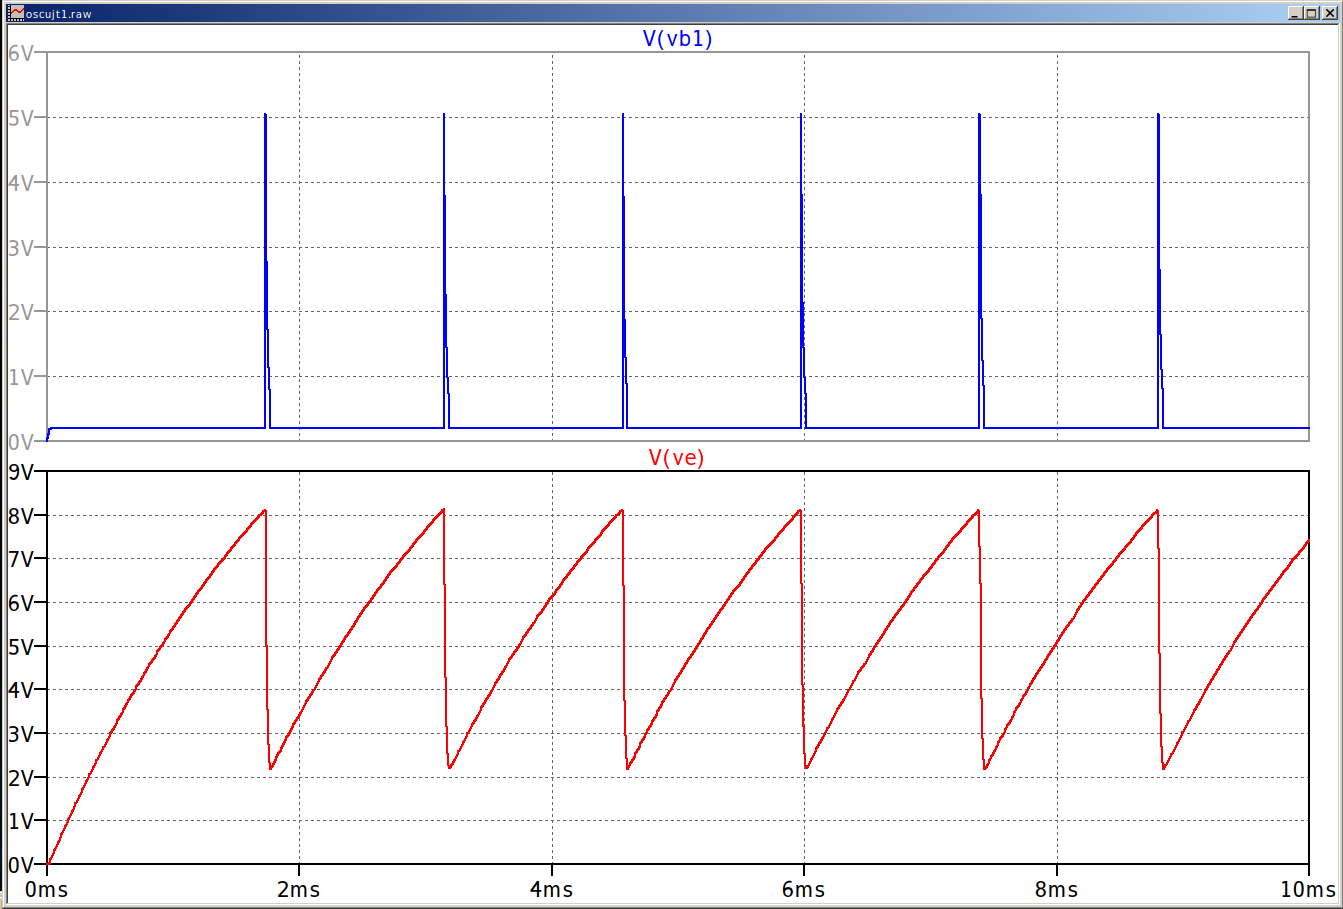
\includegraphics[width=0.8\linewidth]{figuras/oscujt_curva.png}
    	\caption{Simulación temporal del circuito de la figura \ref{ujt1}.}
    	\label{ujt2}
    \end{figure}
    
    \section{Fuentes controladas especiales}
    
  {\hspace{10pt}} Mediante la utilización de las fuentes de tensión y de corriente \emph{Behavioral} disponibles en LTSpice se pueden modelizar comportamientos más complejos de dispositivos y sistemas electrónicos, un ejemplo de ello es la fuente de corriente $B_1$ mostrada en el macromodelo del operacional LM741 en la figura \ref{oper3}, en ese caso $B_1$ depende de 5 corrientes diferentes presentes en el circuito.
  
  En la figura \ref{especial1} se muestran dos ejemplos de fuentes de tensión controladas \emph{Behavioral}, $B_1$ y $B_2$. El caso de $B_1$ utiliza la función \emph{if(a,b,c)} ($if\quad a, \quad then \quad b, \quad else \quad c $) en forma anidada para implementar un amplificador de tensión de ganancia 10 y saturación en $\pm 10V$, en el gráfico inferior de  la figura \ref{especial2} se muestra su transferencia. $B_2$ utiliza la función definida por puntos \emph{table} para implementar un amplificador lineal por tramos con saturación, la transferencia se muestra en el gráfico superior de la figura \ref{especial2}.
  
  Del mismo modo que en el caso anterior se pueden utilizar fuentes de corriente controladas \emph{Behavioral}, en forma particular los circuitos de la figura \ref{especial3} muestran  fuentes de corriente controladas por su propia tensión en bornes para simular impedancias no lineales. En el caso de $B_1$ se implementa una función definida por puntos y en el caso $B_2$ una función matemática específica. 
  
  En la figura \ref{especial4} se muestran las transferencias correspondientes mostrando ambas comportamiento de impedancias diferenciales negativas.
  
  Una aplicación posible de estas impedancias no lineales es en el análisis del bien conocido circuito  con comportamiento caótico de Chua  \cite{chua1990}. Dicho circuito necesita un dispositivo con zonas de resistencia diferencial negativa denominado diodo de Chua. En la figura \ref{especial5} se muestra el circuito con una fuente de corriente controlada $B_1$ que se comporta del modo ya descripto.
  
  
  Para visualizar el comportamiento del circuito se muestran los resultados de la simulación temporal de las variables de estado $V(a)$ e $I(L_1)$ en la figura \ref{especial6} y el plano de fase de ambas variables en la figura \ref{especial7}, revelando el mencionado comportamiento caótico.
  
   \begin{figure}
  	\centering
  	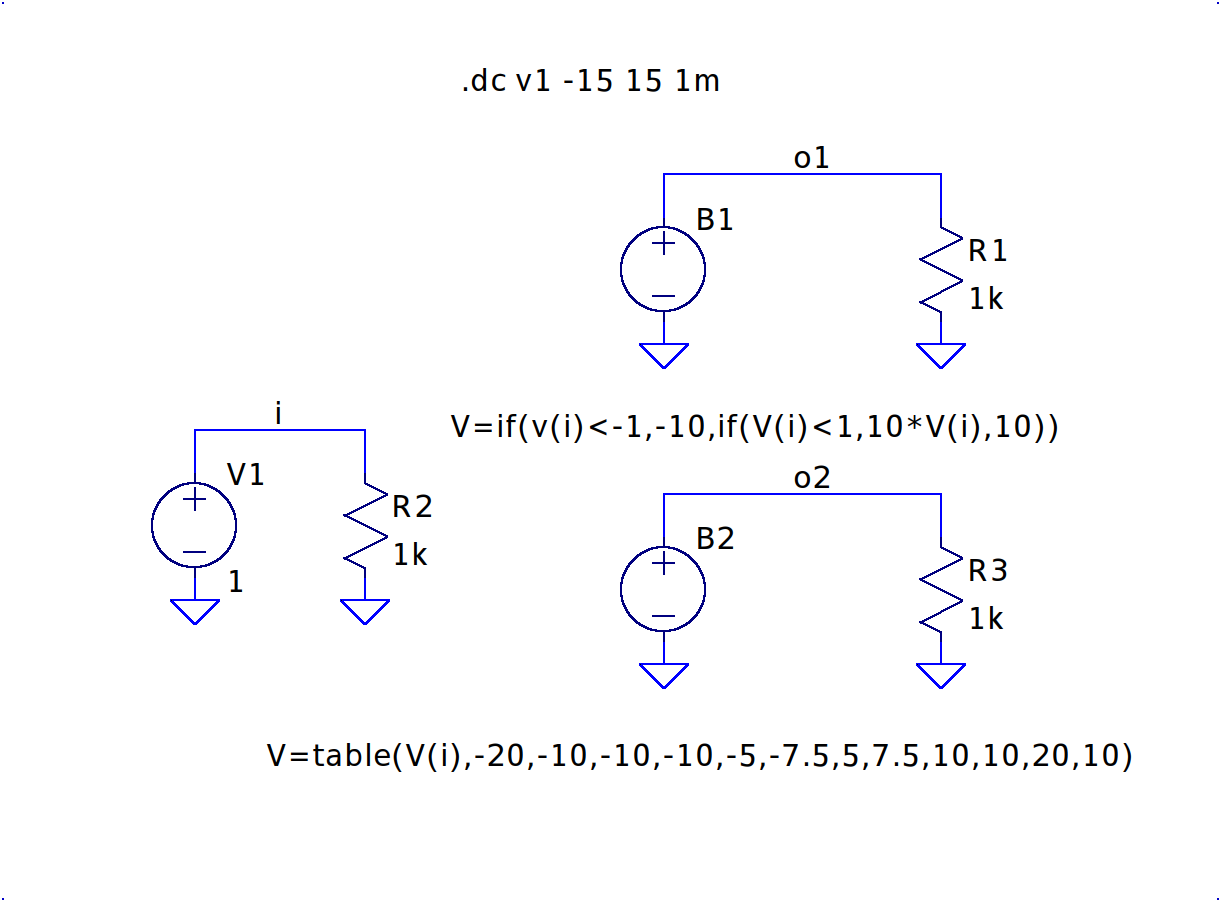
\includegraphics[width=0.8\linewidth]{figuras/especial1_circuito.png}
  	\caption{Implementación de transferencias con fuentes de tensión \emph{Behavioral} controladas. }
  	\label{especial1}
  \end{figure}
  
  \begin{figure}
  	\centering
  	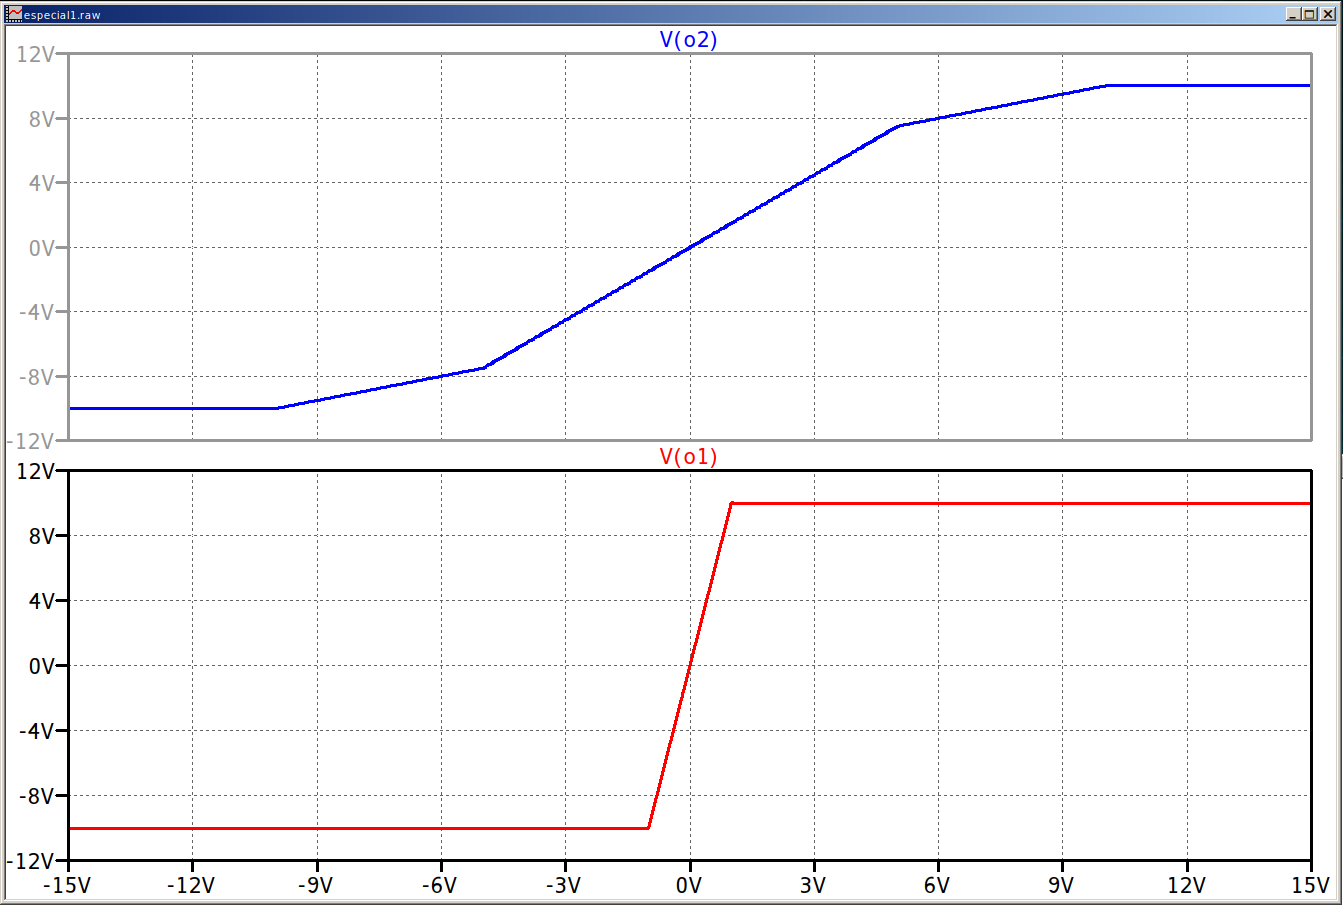
\includegraphics[width=0.8\linewidth]{figuras/especial1_curva.png}
  	\caption{Simulación de las transferencias de los circuitos de la figura \ref{especial1}.}
  	\label{especial2}
  \end{figure}
  
  
  \begin{figure}
  	\centering
  	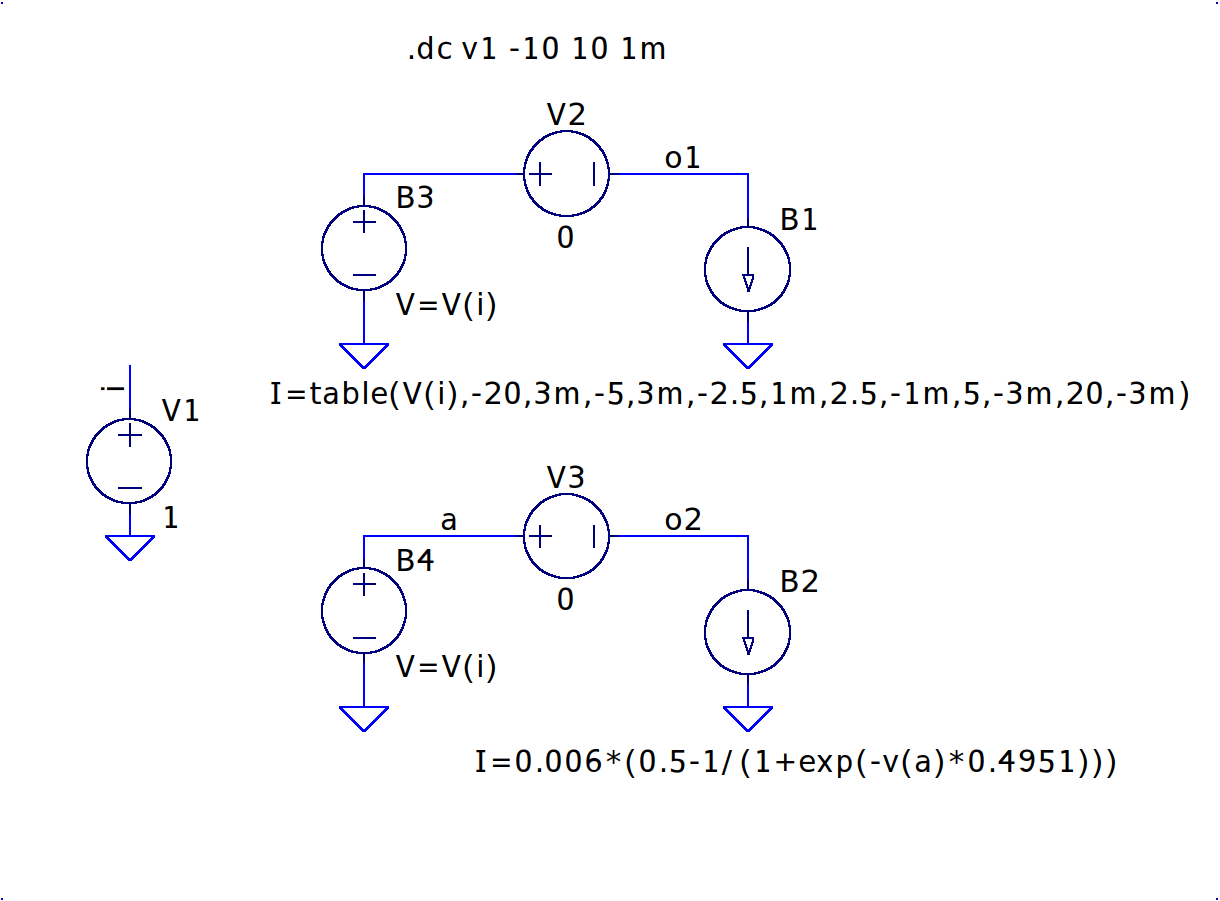
\includegraphics[width=0.8\linewidth]{figuras/especial2_circuito.png}
  	\caption{Implementación de impedancias no lineales con fuentes de corriente \emph{Behavioral} controladas. }
  	\label{especial3}
  \end{figure}
  
  \begin{figure}
  	\centering
  	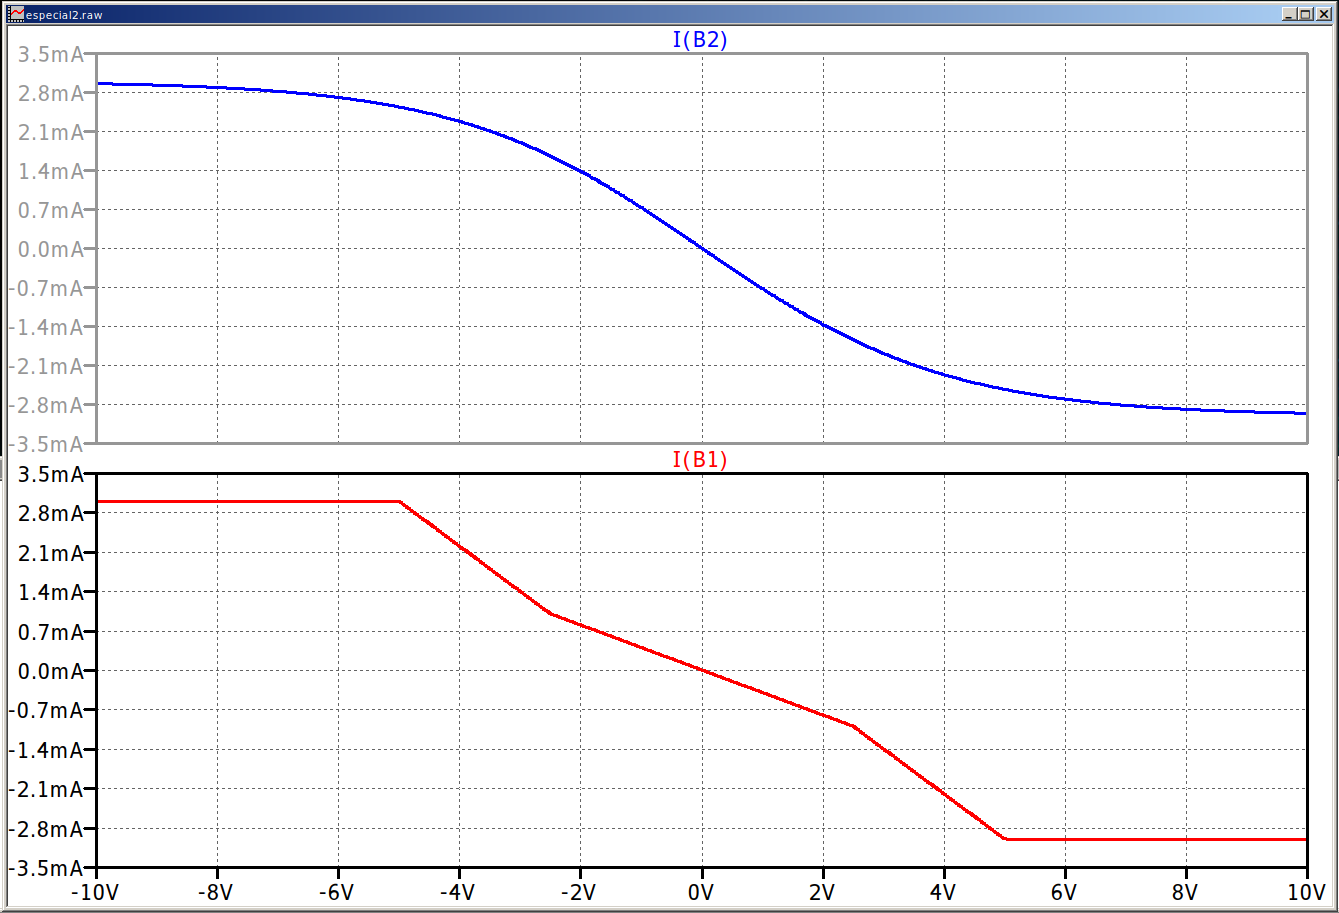
\includegraphics[width=0.8\linewidth]{figuras/especial2_curva.png}
  	\caption{Simulación de las transferencias de los circuitos de la figura \ref{especial2}.}
  	\label{especial4}
  \end{figure}
  
   \begin{figure}
  	\centering
  	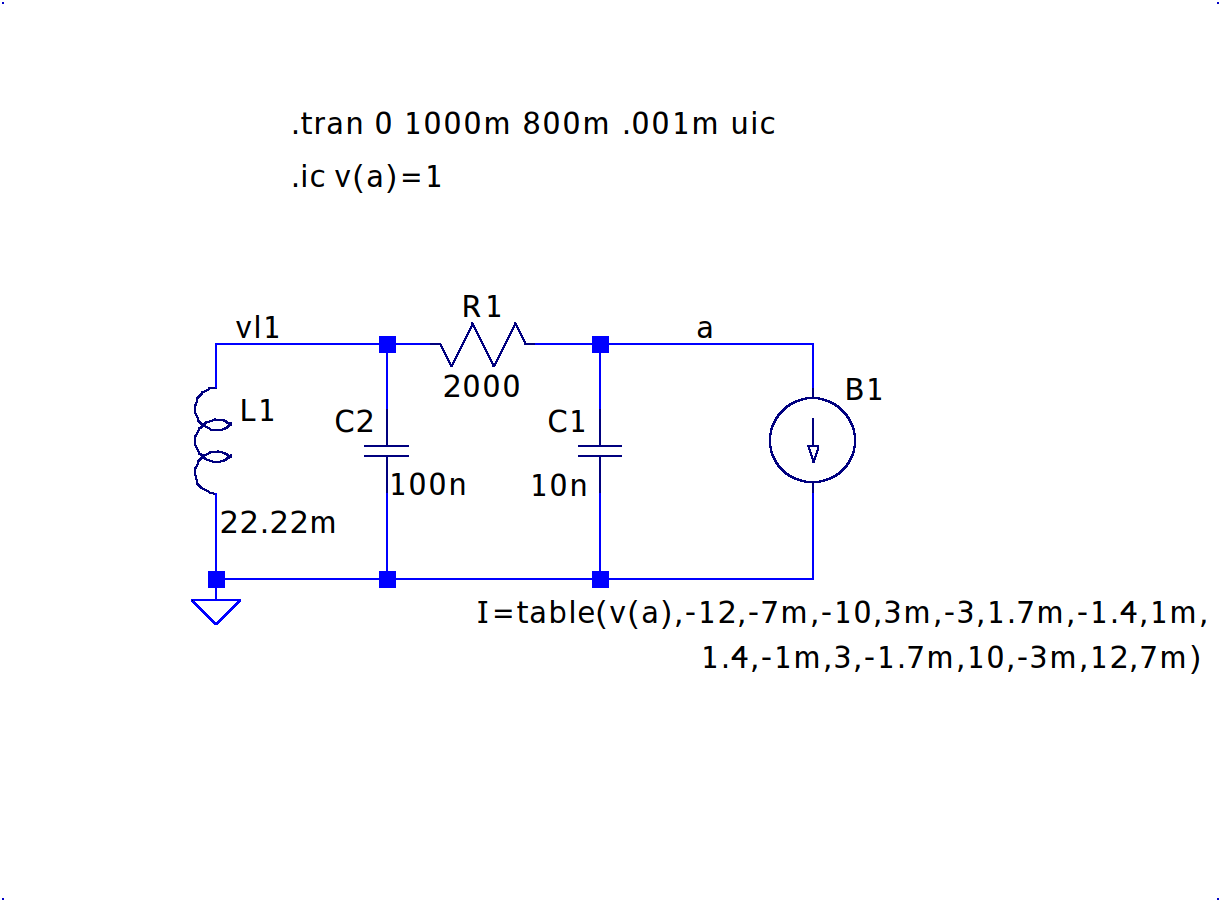
\includegraphics[width=0.8\linewidth]{figuras/especial3_circuito.png}
  	\caption{Circuito de Chua. }
  	\label{especial5}
  \end{figure}
  
  \begin{figure}
  	\centering
  	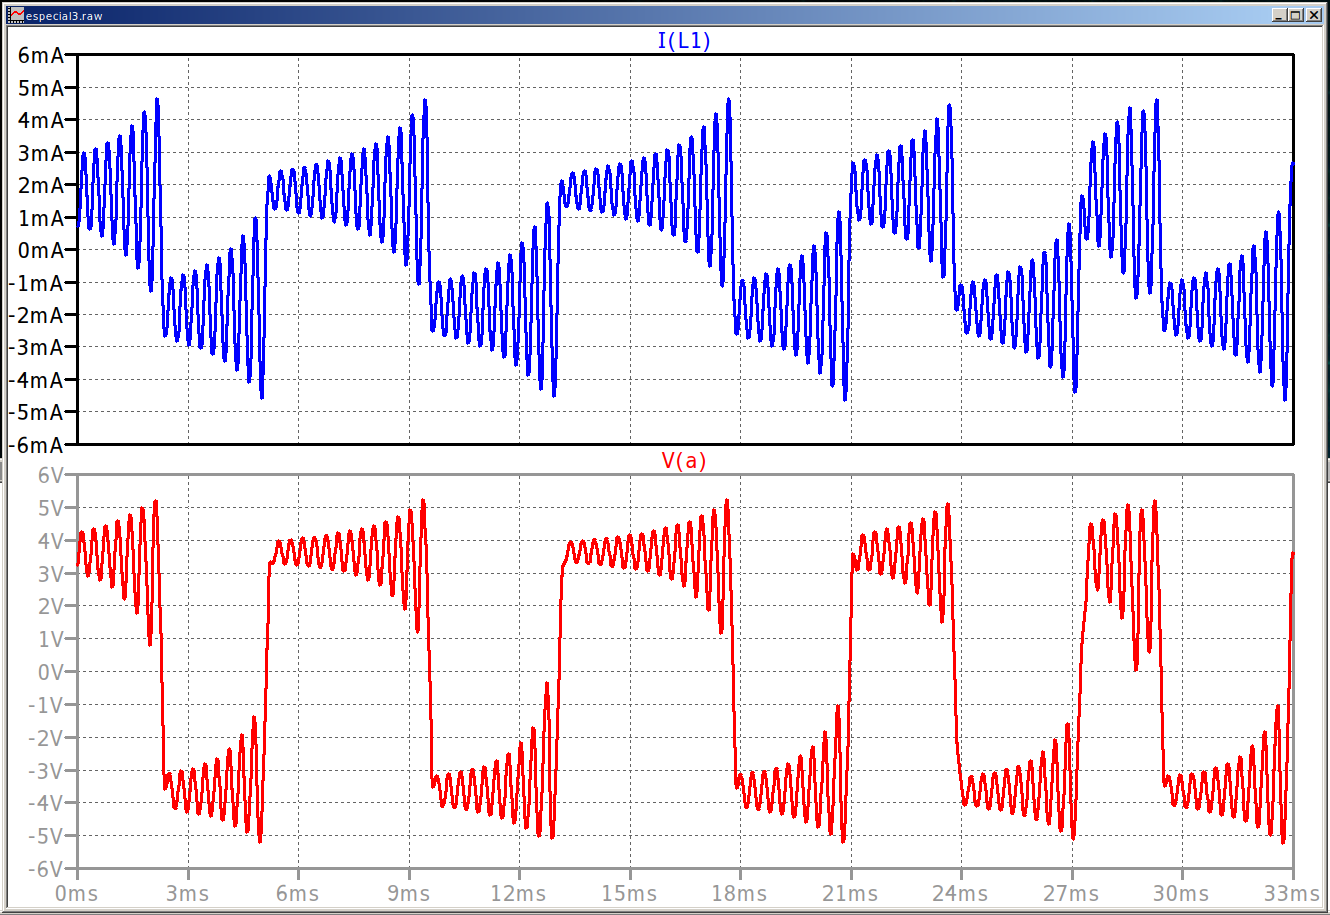
\includegraphics[width=0.8\linewidth]{figuras/especial3_curva1.png}
  	\caption{Simulación temporal del circuito de la figura \ref{especial5}.}
  	\label{especial6}
  \end{figure}
  
  \begin{figure}
  	\centering
  	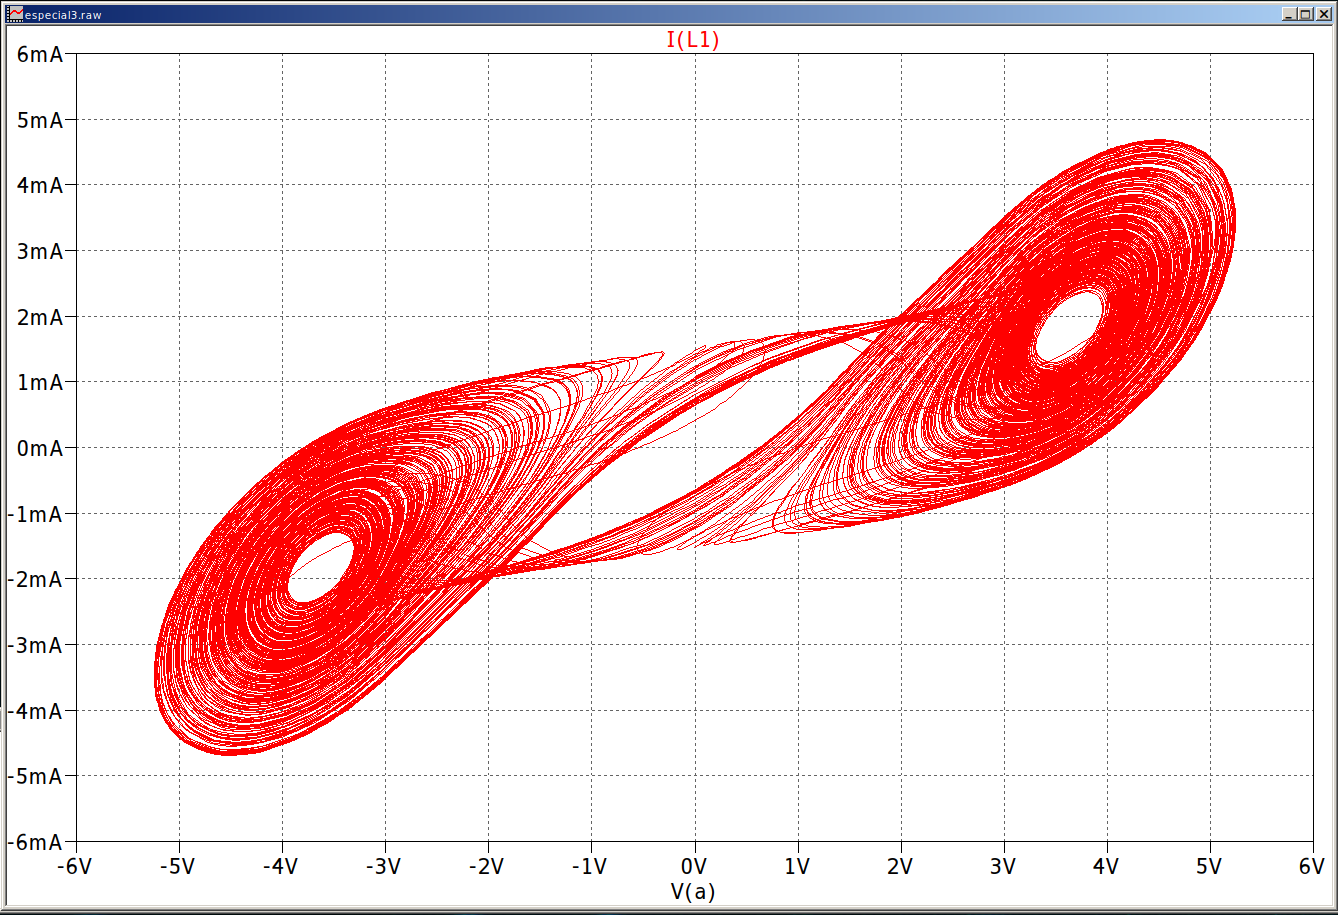
\includegraphics[width=0.8\linewidth]{figuras/especial3_curva2.png}
  	\caption{Plano de fase del circuito de la figura \ref{especial5}.}
  	\label{especial7}
  \end{figure}